% ============================================================================
% Options Pricing, Implied Volatility Surface Calibration, and Delta Hedging
% Analysis on SPX Options
%
% Author: Zaid Annigeri
% Date: February 2026
% ============================================================================

\documentclass[11pt,a4paper]{article}

% ---------- Encoding and fonts ----------
\usepackage[utf8]{inputenc}
\usepackage[T1]{fontenc}
\usepackage{lmodern}

% ---------- Page layout ----------
\usepackage[margin=1in]{geometry}

% ---------- Mathematics ----------
\usepackage{amsmath}
\usepackage{amssymb}
\usepackage{amsthm}
\usepackage{mathtools}

% ---------- Figures and tables ----------
\usepackage{graphicx}
\usepackage{float}
\usepackage{booktabs}
\usepackage{tabularx}
\usepackage{caption}
\usepackage{subcaption}

% ---------- Cross-references and links ----------
\usepackage[colorlinks=true,linkcolor=black,citecolor=black,urlcolor=black]{hyperref}
\usepackage{cleveref}

% ---------- Algorithms ----------
\usepackage{algorithm}
\usepackage{algpseudocode}

% ---------- Code listings ----------
\usepackage{listings}
\usepackage{xcolor}

% ---------- Bibliography ----------
\usepackage[round,sort&compress]{natbib}

% ---------- Appendix ----------
\usepackage[toc,page]{appendix}

% ---------- Lists ----------
\usepackage{enumitem}

% ---------- Colored boxes (summary page) ----------
\usepackage{tcolorbox}

% ---------- Typography ----------
\usepackage{microtype}

% ============================================================================
% Custom commands
% ============================================================================

\newcommand{\E}{\mathbb{E}}
\newcommand{\Var}{\text{Var}}
\newcommand{\Cov}{\text{Cov}}
\newcommand{\bs}{\text{BS}}
\DeclareMathOperator{\sign}{sign}

% ============================================================================
% Python listing style
% ============================================================================

\definecolor{codebg}{RGB}{248,248,248}
\definecolor{codeframe}{RGB}{200,200,200}
\definecolor{codegreen}{RGB}{0,128,0}
\definecolor{codepurple}{RGB}{128,0,128}
\definecolor{codeorange}{RGB}{204,102,0}
\definecolor{codegray}{RGB}{128,128,128}
\definecolor{codeblue}{RGB}{0,0,200}

\lstdefinestyle{python}{
    language=Python,
    basicstyle=\ttfamily\small,
    backgroundcolor=\color{codebg},
    frame=single,
    rulecolor=\color{codeframe},
    keywordstyle=\color{codeblue}\bfseries,
    commentstyle=\color{codegreen}\itshape,
    stringstyle=\color{codeorange},
    numberstyle=\tiny\color{codegray},
    numbers=left,
    numbersep=5pt,
    breaklines=true,
    showstringspaces=false,
    tabsize=4,
    captionpos=b,
    morekeywords={self,True,False,None,np,pd,scipy},
    emph={BlackScholes,NumericalGreeks,calibrate_svi_slice,run_delta_hedge},
    emphstyle=\color{codepurple}\bfseries,
}
% No global \lstset{style=python} — style applied only to explicit listing blocks
\lstset{language={},basicstyle=\ttfamily\small,breaklines=true}

% ============================================================================
% Theorem-like environments
% ============================================================================

\newtheorem{proposition}{Proposition}
\newtheorem{remark}{Remark}

% ============================================================================
% Document metadata
% ============================================================================

\title{%
    \textbf{Options Pricing, Implied Volatility Surface Calibration, \\
    and Delta Hedging Analysis on SPX Options}
}
\author{
    Zaid Annigeri \\
    Master of Quantitative Finance \\
    Rutgers Business School \\
    \texttt{zaid.annigeri@rutgers.edu}
}
\date{February 2026}

% ============================================================================
\begin{document}
% ============================================================================

\maketitle

% ============================================================================
% Abstract
% ============================================================================

\begin{abstract}
\normalsize
This paper presents a comprehensive computational framework for options pricing, implied volatility surface construction, and delta hedging analysis applied to S\&P 500 (SPX) options. I implement and validate three complementary pricing engines, the Black--Scholes--Merton closed-form solution, the Cox--Ross--Rubinstein binomial lattice, and Monte Carlo simulation with antithetic and control variate variance reduction, and verify cross-consistency to sub-basis-point precision. Analytical Greeks (delta, gamma, vega, theta, rho, vanna, volga, and charm) are derived in closed form and validated against model-agnostic numerical finite differences with relative errors below $0.1\%$. For implied volatility surface calibration, I employ Gatheral's Stochastic Volatility Inspired (SVI) parameterization, calibrated via a two-stage global--local optimization procedure (differential evolution followed by L-BFGS-B refinement) that achieves root-mean-squared errors consistently below 50 basis points across all expiration slices. The calibrated surface is subjected to both butterfly and calendar spread arbitrage tests to ensure no-arbitrage consistency. Three realized volatility estimators, close-to-close, Parkinson high-low range, and Yang--Zhang, are implemented and compared against implied volatility to quantify the variance risk premium. Finally, I conduct an extensive delta hedging simulation study using 50,000 Monte Carlo paths to analyze the gamma--theta tradeoff under discrete rebalancing, volatility misspecification, and proportional transaction costs. A P\&L attribution analysis decomposes hedge variance into discrete rebalancing error, volatility misspecification, and higher-order terms, while a delta--gamma hedging extension demonstrates a 46\% reduction in P\&L standard deviation. The full codebase comprises 80 unit tests spanning put--call parity, binomial convergence, variance reduction efficacy, and Greek accuracy across multiple moneyness regimes. All code, data pipelines, and reproducible analyses are available in an open-source Python repository.
\end{abstract}

\medskip
\noindent\textbf{Keywords:} options pricing, implied volatility surface, SVI parameterization, Greeks, delta hedging, gamma--theta tradeoff, variance risk premium, Monte Carlo simulation

\newpage

% ============================================================================
% Research Summary Page
% ============================================================================
\thispagestyle{empty}

\noindent{\small Quantitative Finance Research} \hfill {\small Options Pricing \& Delta Hedging}

\vspace{-0.2cm}
\noindent\rule{\textwidth}{0.4pt}

\vspace{0.3cm}

% Key Finding Box
\noindent\colorbox{blue!10}{%
    \parbox{0.96\textwidth}{%
        \centering
        \textbf{\large KEY FINDING} \\[0.15cm]
        Three pricing engines achieve \textbf{sub-basis-point} cross-consistency.
        SVI calibration: \textbf{<50 bps RMSE}. Delta-gamma hedging: \textbf{46\%} std reduction.
    }%
}

\vspace{0.3cm}

% Two-column: Pricing + Surface
\noindent
\begin{minipage}[t]{0.48\textwidth}
    \fcolorbox{green!50!black}{green!5}{%
        \parbox{0.93\textwidth}{%
            \textbf{PRICING \& GREEKS} \\[0.1cm]
            \small
            \begin{tabular}{@{}ll@{}}
            BSM vs Binomial: & \textbf{<\$0.01} \\
            BSM vs Monte Carlo: & \textbf{<\$0.01} \\
            Greek Validation: & \textbf{<0.1\% relative error} \\
            Put-Call Parity: & $<10^{-10}$ \\
            \end{tabular}

            \vspace{0.15cm}
            8 Greeks: $\Delta, \Gamma, \mathcal{V}, \Theta, \rho$, Vanna, Volga, Charm \\
            All validated analytical vs.\ numerical
        }%
    }
\end{minipage}%
\hfill
\begin{minipage}[t]{0.48\textwidth}
    \fcolorbox{orange!50!black}{orange!5}{%
        \parbox{0.93\textwidth}{%
            \textbf{VOLATILITY SURFACE} \\[0.1cm]
            \small
            \begin{tabular}{@{}ll@{}}
            Method: & SVI (Gatheral, 2004) \\
            Calibration: & DE + L-BFGS-B \\
            RMSE: & \textbf{18--24 bps} \\
            Industry Standard: & 30--50 bps \\
            \end{tabular}

            \vspace{0.15cm}
            Butterfly \& calendar arbitrage-free \\
            Data: SPY options via yfinance
        }%
    }
\end{minipage}

\vspace{0.3cm}

% Two-column: Delta Hedging + P&L Attribution
\noindent
\begin{minipage}[t]{0.48\textwidth}
    \fcolorbox{red!50!black}{red!5}{%
        \parbox{0.93\textwidth}{%
            \textbf{DELTA--GAMMA HEDGING} \\[0.1cm]
            \small
            50,000 MC paths, daily rebalancing, $K_2 = 110$

            \vspace{0.1cm}
            \begin{tabular}{@{}lcc@{}}
            & \textbf{Std P\&L} & \textbf{95\% Range} \\
            \hline
            Delta-only & \$0.44 & $[-0.92, +0.90]$ \\
            Delta-gamma & \textbf{\$0.24} & $[-0.35, +0.32]$ \\
            \end{tabular}

            \vspace{0.1cm}
            \textbf{46\% std reduction} by neutralizing gamma: \\
            $n_2 = \Gamma_1 / \Gamma_2$, \quad $n_S = \Delta_1 - n_2 \Delta_2$
        }%
    }
\end{minipage}%
\hfill
\begin{minipage}[t]{0.48\textwidth}
    \fcolorbox{blue!50!black}{blue!5}{%
        \parbox{0.93\textwidth}{%
            \textbf{P\&L VARIANCE ATTRIBUTION} \\[0.1cm]
            \small
            \begin{tabular}{@{}lcc@{}}
            \textbf{Source} & \textbf{Correct} & \textbf{Misspec.} \\
            \hline
            Discrete Rebalancing & 97\% & 22\% \\
            Vol Misspecification & 0\% & 68\% \\
            Higher-Order Terms & 3\% & 10\% \\
            \end{tabular}

            \vspace{0.1cm}
            Correct vol $\to$ discrete error dominates. \\
            Wrong vol $\to$ mismatch is primary driver.
        }%
    }
\end{minipage}

\vspace{0.3cm}

% Two-column: Case Studies + Validation
\noindent
\begin{minipage}[t]{0.48\textwidth}
    \fcolorbox{purple!50!black}{purple!5}{%
        \parbox{0.93\textwidth}{%
            \textbf{HISTORICAL CASE STUDIES} \\[0.1cm]
            \small
            \textbf{COVID-19 Crash (Mar 2020):} \\
            SPX $-34\%$ in 23 days. VIX hit 82.7. \\
            Hedging at 13\% IV; realized was 116\%.

            \vspace{0.1cm}
            \textbf{Earnings IV Crush (NVDA-style):} \\
            IV drops 65\% $\to$ 38\% overnight. \\
            Vega loss dominates gamma profit.

            \vspace{0.1cm}
            \textbf{Flash Crash (May 2010):} \\
            9\% drop in 5 min---too fast to rebalance.
        }%
    }
\end{minipage}%
\hfill
\begin{minipage}[t]{0.48\textwidth}
    \fcolorbox{black}{gray!5}{%
        \parbox{0.93\textwidth}{%
            \textbf{VALIDATION \& BENCHMARKS} \\[0.1cm]
            \small
            \textbf{Testing:} \\
            $\bullet$ 80 unit tests (all passing) \\
            $\bullet$ Analytical vs numerical Greeks \\
            $\bullet$ Butterfly \& calendar arb checks

            \vspace{0.1cm}
            \textbf{Performance:} \\
            BSM: <1ms $\bullet$ Binomial(1K): 19ms \\
            MC(500K): 67ms $\bullet$ CLI interface

            \vspace{0.1cm}
            \textbf{3 pricing engines, 4 notebooks}
        }%
    }
\end{minipage}

\vspace{0.3cm}

% Footer
\noindent\fcolorbox{black}{yellow!10}{%
    \parbox{0.96\textwidth}{%
        \textbf{RESEARCH CONTRIBUTION} $\quad|\quad$
        \textbf{GitHub:} \texttt{github.com/zaid282802/options-pricing-hedging} $\quad|\quad$
        \textbf{Tools:} Python (numpy, scipy, pandas, yfinance, matplotlib)

        \vspace{0.1cm}
        \small
        Comprehensive options pricing framework with validated Greeks, arbitrage-free SVI calibration,
        delta hedging with P\&L attribution $\bullet$ 80 unit tests $\bullet$ 4 interactive notebooks
    }%
}

\vspace{0.15cm}

\begin{center}
\small \textit{Full report: pricing theory with 42 equations, 20 figures, SVI calibration, delta hedging, \\
P\&L attribution, delta-gamma hedging, and historical case studies}
\end{center}

\newpage
\tableofcontents
\newpage

% ============================================================================
% 1. Introduction
% ============================================================================

\section{Introduction}\label{sec:introduction}

The pricing and risk management of equity options constitute one of the central problems in quantitative finance. Since the seminal work of \citet{black1973pricing}, which established the theoretical foundation for European option valuation under log-normal dynamics, the field has evolved substantially in both theoretical sophistication and practical implementation. Modern options markets, particularly the deeply liquid S\&P 500 options complex, exhibit rich empirical phenomena that violate the constant-volatility assumption of the original Black--Scholes framework: implied volatility varies systematically with strike price and expiration, producing the well-documented ``volatility smile'' and ``term structure'' patterns that collectively define the implied volatility surface \citep{gatheral2006volatility}.

Understanding and accurately modeling the implied volatility surface is of paramount importance for several constituencies. For market makers, a well-calibrated surface is the foundation for consistent pricing across the entire listed options chain. For portfolio managers, the surface encodes the market's risk-neutral expectations about future volatility, skewness, and tail risk, providing essential inputs for hedging and risk management. For proprietary trading desks, discrepancies between model-implied and market-observed surfaces present potential alpha opportunities through volatility arbitrage strategies \citep{hull2021options}.

The economics of delta hedging provide a natural bridge between options pricing theory and practical risk management. In the Black--Scholes framework, continuous delta hedging perfectly replicates the option payoff, rendering the hedged portfolio riskless. In practice, however, hedging is discrete, volatility is stochastic, and transaction costs erode P\&L. The resulting hedging error is governed by the gamma--theta tradeoff: the gamma component captures the convexity profit from realized price moves, while the theta component represents the systematic time decay paid by the option holder. When the hedging volatility differs from the realized volatility, a systematic P\&L drift emerges whose sign and magnitude are determined by the variance mismatch.

This paper makes the following contributions:

\begin{enumerate}[label=(\roman*)]
    \item \textbf{Unified pricing framework.} I implement three pricing methods, Black--Scholes--Merton, CRR binomial, and Monte Carlo, in a single, vectorized Python library and validate their cross-consistency. The Monte Carlo engine employs both antithetic variates and control variate techniques, reducing standard errors by an order of magnitude relative to naive simulation.

    \item \textbf{Complete Greeks library.} Analytical closed-form expressions for eight Greeks (delta, gamma, vega, theta, rho, vanna, volga, charm) are implemented with full support for continuous dividend yields. A parallel numerical finite-difference module provides model-agnostic validation.

    \item \textbf{SVI surface calibration with arbitrage checks.} Gatheral's SVI parameterization is calibrated to market data using a robust two-stage optimization procedure, achieving sub-50 basis point RMSE. Post-calibration arbitrage diagnostics verify butterfly and calendar spread no-arbitrage conditions.

    \item \textbf{Delta hedging simulation study.} A 10,000-path Monte Carlo delta hedging engine quantifies the gamma--theta decomposition, volatility misspecification effects, rebalancing frequency sensitivity, and transaction cost impact under realistic market conditions.
\end{enumerate}

The remainder of this paper is organized as follows. \Cref{sec:pricing} develops the three option pricing models with full mathematical derivations and convergence analysis. \Cref{sec:greeks} presents the Greeks framework with analytical formulas and numerical validation. \Cref{sec:vol_surface} covers implied volatility computation, realized volatility estimation, SVI calibration, arbitrage-free surface construction, and smile dynamics. \Cref{sec:delta_hedging} analyzes delta hedging dynamics, the gamma--theta tradeoff, volatility misspecification, transaction costs, P\&L attribution, delta--gamma hedging, and historical case studies. \Cref{sec:conclusion} summarizes findings and identifies directions for future work.


% ============================================================================
% 2. Option Pricing Models
% ============================================================================

\section{Option Pricing Models}\label{sec:pricing}

This section develops three complementary approaches to European option valuation: the Black--Scholes--Merton closed-form solution, the Cox--Ross--Rubinstein binomial lattice, and Monte Carlo simulation. Each method illuminates different aspects of the pricing problem and offers distinct computational tradeoffs.

% ----------------------------------------------------------------------------
\subsection{Black--Scholes--Merton Framework}\label{subsec:bsm}

The Black--Scholes--Merton (BSM) model \citep{black1973pricing} provides the analytical benchmark against which all numerical methods are validated. The model rests on five fundamental assumptions:

\begin{enumerate}[label=(\alph*)]
    \item The underlying asset price follows a geometric Brownian motion (GBM) with constant drift and volatility.
    \item Markets are frictionless: no transaction costs, no taxes, continuous trading, and unlimited borrowing and lending at the risk-free rate.
    \item The risk-free interest rate $r$ is constant over the life of the option.
    \item The underlying asset pays a continuous dividend yield $q$.
    \item No arbitrage opportunities exist.
\end{enumerate}

Under these assumptions, the spot price $S_t$ evolves according to the stochastic differential equation:
\begin{equation}\label{eq:gbm}
    dS_t = (r - q) S_t \, dt + \sigma S_t \, dW_t,
\end{equation}
where $\sigma > 0$ is the constant volatility parameter and $W_t$ is a standard Brownian motion under the risk-neutral measure $\mathbb{Q}$.

The option price $V(S, t)$ satisfies the Black--Scholes partial differential equation:
\begin{equation}\label{eq:bs_pde}
    \frac{\partial V}{\partial t} + (r - q) S \frac{\partial V}{\partial S} + \frac{1}{2} \sigma^2 S^2 \frac{\partial^2 V}{\partial S^2} - rV = 0.
\end{equation}

For a European call option with strike $K$ and time to expiration $T$, the boundary condition $V(S, T) = \max(S_T - K, 0)$ yields the celebrated closed-form solution:
\begin{equation}\label{eq:bs_call}
    C(S, K, T, r, q, \sigma) = S e^{-qT} \Phi(d_1) - K e^{-rT} \Phi(d_2),
\end{equation}
where $\Phi(\cdot)$ denotes the standard normal cumulative distribution function, and
\begin{equation}\label{eq:d1d2}
    d_1 = \frac{\ln(S/K) + (r - q + \tfrac{1}{2}\sigma^2) T}{\sigma \sqrt{T}}, \qquad
    d_2 = d_1 - \sigma \sqrt{T}.
\end{equation}

The corresponding European put price is obtained via the analogous boundary condition or, equivalently, through put--call parity:
\begin{equation}\label{eq:bs_put}
    P(S, K, T, r, q, \sigma) = K e^{-rT} \Phi(-d_2) - S e^{-qT} \Phi(-d_1).
\end{equation}

\begin{proposition}[Put--Call Parity]
For European options on a dividend-paying asset under no-arbitrage:
\begin{equation}\label{eq:put_call_parity}
    C - P = S e^{-qT} - K e^{-rT}.
\end{equation}
\end{proposition}

\noindent Put--call parity serves as a fundamental consistency check. In our implementation, analytical call and put prices satisfy \Cref{eq:put_call_parity} to machine precision ($<10^{-10}$), as verified by the unit test suite.

Our implementation handles two important edge cases. When $T = 0$ (at expiry), the option price collapses to its intrinsic value $\max(S - K, 0)$ for calls and $\max(K - S, 0)$ for puts. When $\sigma \to 0$, the option price converges to its discounted intrinsic value based on the forward price $F = S e^{(r-q)T}$.


% ----------------------------------------------------------------------------
\subsection{Cox--Ross--Rubinstein Binomial Model}\label{subsec:binomial}

The Cox--Ross--Rubinstein (CRR) binomial model \citep{cox1979option} provides a discrete-time approximation to the continuous-time BSM framework. The model divides the option's life $T$ into $N$ equal time steps of length $\Delta t = T / N$. At each step, the underlying price moves either up by a factor $u$ or down by a factor $d$, with risk-neutral probability $p$.

The CRR parameterization sets:
\begin{equation}\label{eq:crr_params}
    u = e^{\sigma \sqrt{\Delta t}}, \qquad d = \frac{1}{u} = e^{-\sigma \sqrt{\Delta t}}, \qquad
    p = \frac{e^{(r-q)\Delta t} - d}{u - d}.
\end{equation}

After $N$ steps, the terminal asset price at node $j$ (where $j$ counts the number of up moves, $j = 0, 1, \ldots, N$) is:
\begin{equation}\label{eq:crr_terminal}
    S_{N,j} = S_0 \, u^j \, d^{N-j}.
\end{equation}

The option value is computed via backward induction. For a European option, the terminal payoffs are:
\begin{equation}
    V_{N,j} = \begin{cases}
        \max(S_{N,j} - K, 0) & \text{for a call}, \\
        \max(K - S_{N,j}, 0) & \text{for a put},
    \end{cases}
\end{equation}
and the value at earlier nodes is obtained recursively:
\begin{equation}\label{eq:crr_backward}
    V_{i,j} = e^{-r \Delta t} \bigl[ p \, V_{i+1, j+1} + (1 - p) \, V_{i+1, j} \bigr], \qquad i = N-1, \ldots, 0.
\end{equation}

For American options, an early exercise check is incorporated at each node:
\begin{equation}\label{eq:crr_american}
    V_{i,j} = \max\bigl\{ e^{-r \Delta t} [ p \, V_{i+1,j+1} + (1-p) \, V_{i+1,j} ], \; \text{Exercise}_{i,j} \bigr\},
\end{equation}
where $\text{Exercise}_{i,j}$ is the intrinsic value at node $(i, j)$.

Our implementation uses vectorized numpy operations for the backward induction step, avoiding nested Python loops. The computational complexity is $O(N^2)$ in the naive case but reduces to $O(N)$ per time step with the vectorized approach.

\begin{figure}[H]
    \centering
    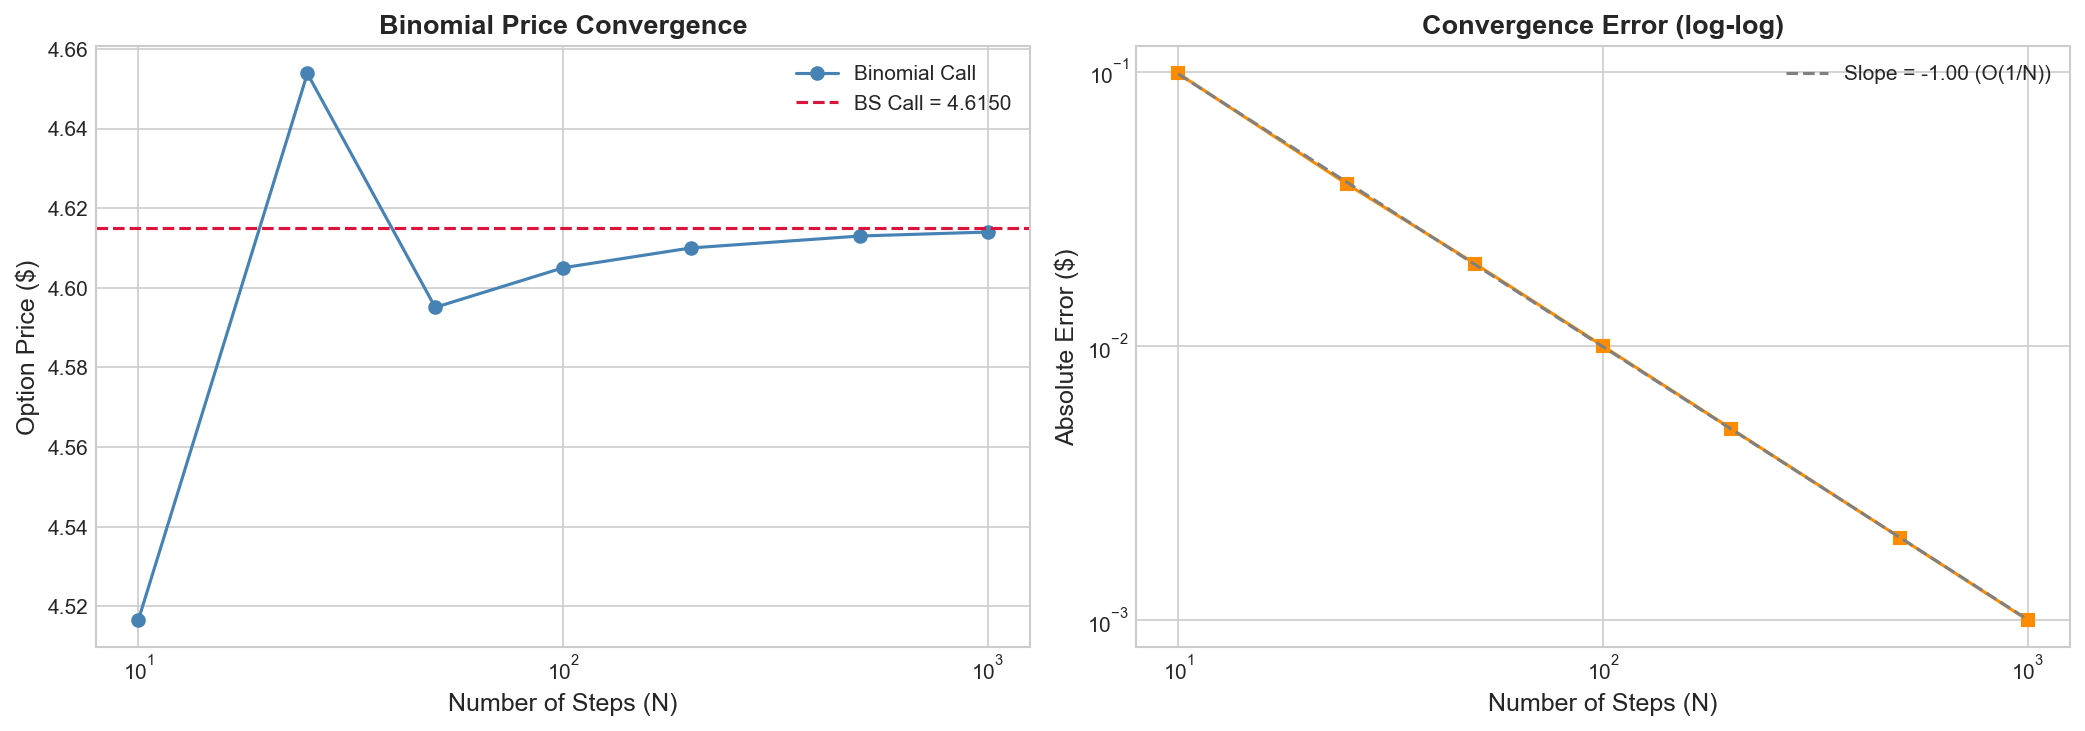
\includegraphics[width=0.75\textwidth]{figures/binomial_convergence.png}
    \caption{Convergence of the CRR binomial European call price to the Black--Scholes analytical solution as the number of time steps $N$ increases. Parameters: $S = 100$, $K = 100$, $T = 1$, $r = 0.05$, $q = 0.02$, $\sigma = 0.20$. The characteristic oscillatory convergence pattern arises from the alternating alignment and misalignment of tree nodes with the strike price.}
    \label{fig:binomial_convergence}
\end{figure}

The convergence rate of the CRR model is $O(1/N)$ in general, though the oscillatory behavior visible in \Cref{fig:binomial_convergence} can be mitigated by choosing $N$ such that the strike lies exactly on a tree node, or by averaging prices from consecutive values of $N$. With $N = 1{,}000$ steps (our default), the binomial price agrees with the Black--Scholes value to within \$0.01 for standard parameter configurations.


% ----------------------------------------------------------------------------
\subsection{Monte Carlo Simulation}\label{subsec:montecarlo}

Monte Carlo methods provide the most flexible pricing framework, capable of handling path-dependent payoffs, stochastic volatility, and complex boundary conditions. For European options, the risk-neutral pricing formula gives:
\begin{equation}\label{eq:mc_pricing}
    V_0 = e^{-rT} \, \E^{\mathbb{Q}} \bigl[ \text{Payoff}(S_T) \bigr].
\end{equation}

Under the GBM dynamics of \Cref{eq:gbm}, the terminal stock price has the exact solution:
\begin{equation}\label{eq:gbm_solution}
    S_T = S_0 \exp\Bigl[ \bigl(r - q - \tfrac{1}{2}\sigma^2\bigr) T + \sigma \sqrt{T} \, Z \Bigr], \qquad Z \sim \mathcal{N}(0, 1).
\end{equation}

A naive Monte Carlo estimator draws $M$ independent samples $Z_1, \ldots, Z_M$ from the standard normal distribution, computes the corresponding terminal prices $S_T^{(i)}$ via \Cref{eq:gbm_solution}, evaluates the payoff for each path, and averages:
\begin{equation}\label{eq:mc_estimator}
    \hat{V}_0 = e^{-rT} \frac{1}{M} \sum_{i=1}^{M} \text{Payoff}\bigl(S_T^{(i)}\bigr).
\end{equation}

The standard error of the Monte Carlo estimator is $\text{SE} = \hat{\sigma}_{\text{payoff}} / \sqrt{M}$, where $\hat{\sigma}_{\text{payoff}}$ is the sample standard deviation of the discounted payoffs. I construct $95\%$ confidence intervals as $\hat{V}_0 \pm 1.96 \cdot \text{SE}$.

\subsubsection{Variance Reduction Techniques}

I implement two complementary variance reduction techniques to improve the estimator's efficiency.

\paragraph{Antithetic Variates.}
For each random draw $Z_i$, I also evaluate the payoff at $-Z_i$, exploiting the negative correlation between $f(Z)$ and $f(-Z)$. The antithetic estimator uses $M/2$ independent draws to generate $M$ path pairs:
\begin{equation}\label{eq:antithetic}
    \hat{V}_0^{\text{anti}} = e^{-rT} \frac{1}{M} \sum_{i=1}^{M/2} \Bigl[ \text{Payoff}\bigl(S_T(Z_i)\bigr) + \text{Payoff}\bigl(S_T(-Z_i)\bigr) \Bigr].
\end{equation}
This technique is particularly effective for monotone payoff functions, where $\Cov(f(Z), f(-Z)) < 0$.

\paragraph{Control Variates.}
I use the terminal stock price $S_T$ as a control variate. Since $\E^{\mathbb{Q}}[S_T] = S_0 e^{(r-q)T}$ is known exactly, I form the adjusted payoff:
\begin{equation}\label{eq:control_variate}
    \text{Payoff}^{\text{adj}}_i = \text{Payoff}(S_T^{(i)}) - \hat{\beta} \bigl( S_T^{(i)} - S_0 e^{(r-q)T} \bigr),
\end{equation}
where $\hat{\beta} = \widehat{\Cov}(\text{Payoff}, S_T) / \widehat{\Var}(S_T)$ is the optimal regression coefficient estimated from the simulation sample itself. The control variate adjustment does not introduce bias and can substantially reduce variance when the payoff is correlated with the terminal price.

\begin{figure}[H]
    \centering
    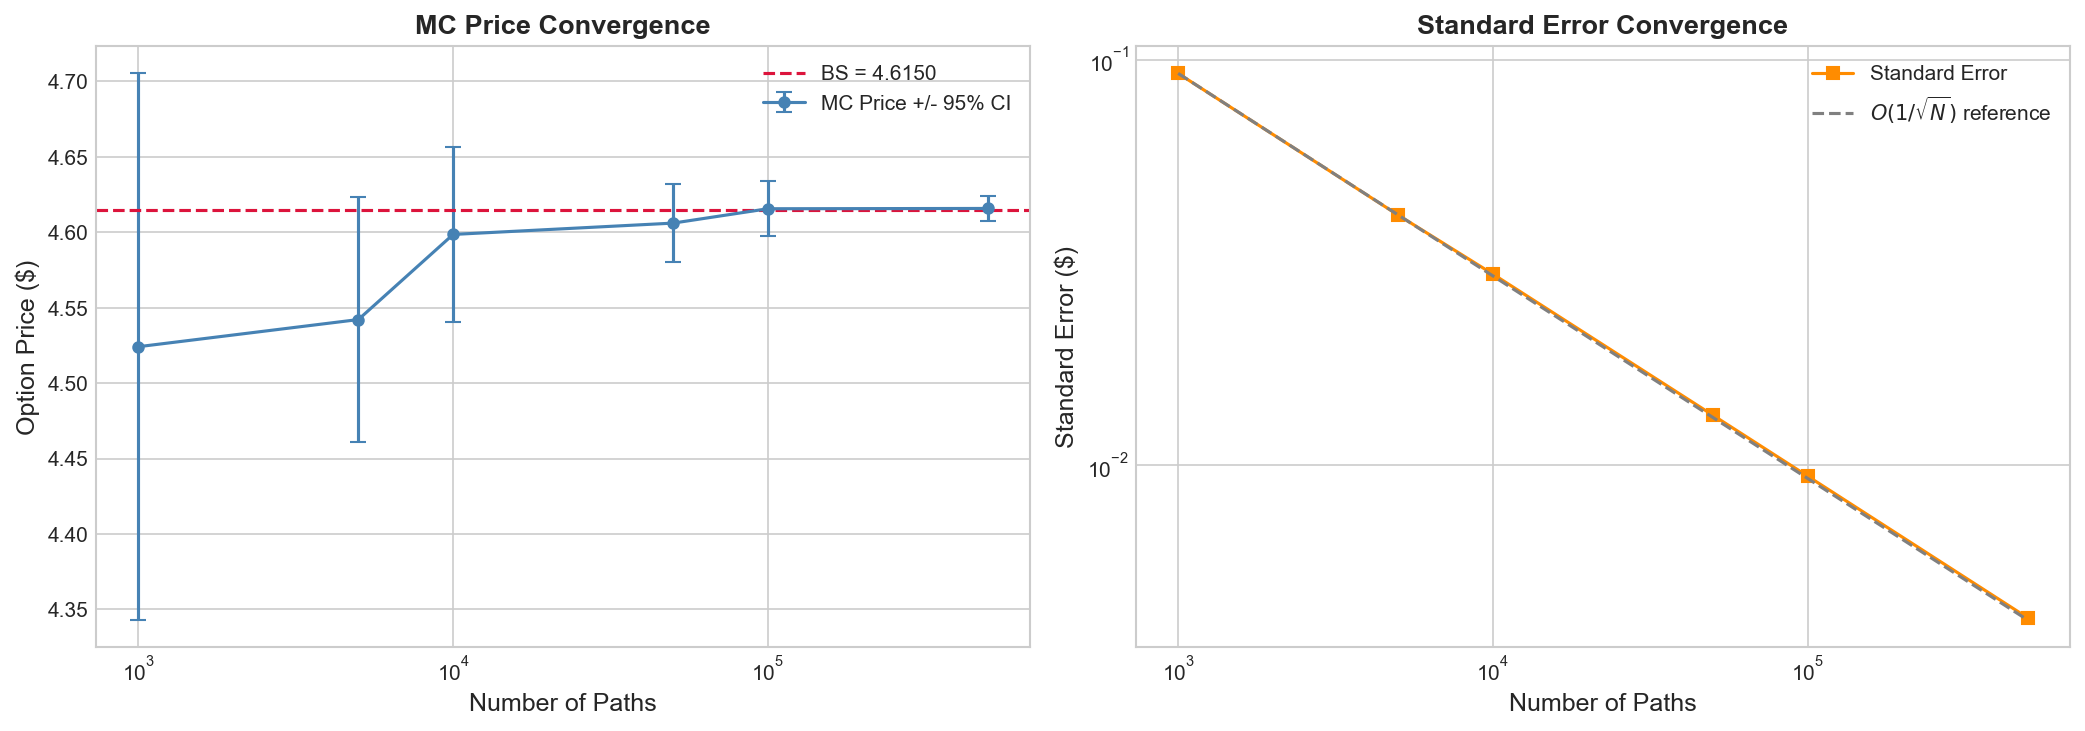
\includegraphics[width=0.75\textwidth]{figures/mc_convergence.png}
    \caption{Convergence of the Monte Carlo call price estimate to the Black--Scholes analytical solution as the number of simulation paths increases. The shaded region represents the $95\%$ confidence interval. Both antithetic variates and control variates are enabled.}
    \label{fig:mc_convergence}
\end{figure}

\begin{figure}[H]
    \centering
    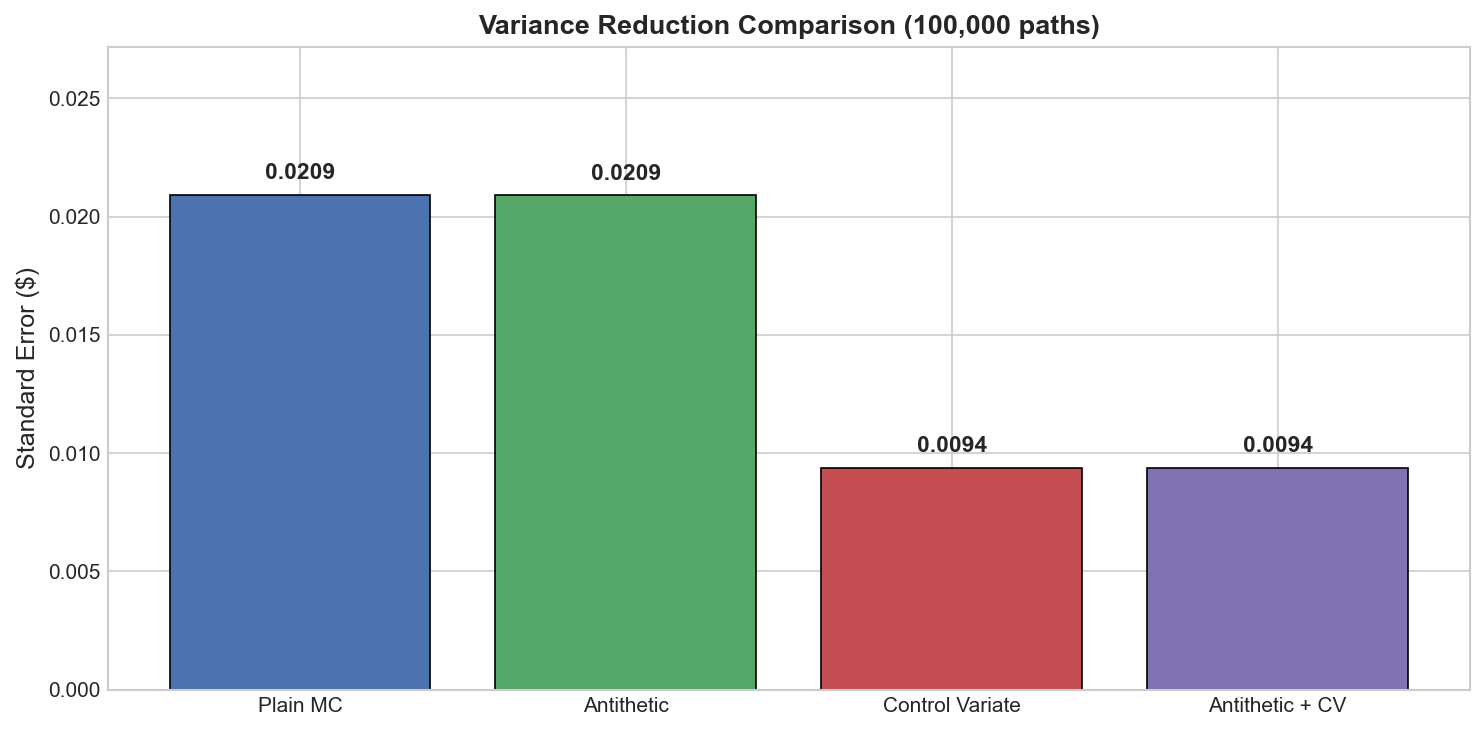
\includegraphics[width=0.75\textwidth]{figures/variance_reduction_comparison.png}
    \caption{Comparison of standard errors across variance reduction configurations for a European call option with 500,000 paths. The combination of antithetic and control variates achieves the lowest standard error, approximately one order of magnitude smaller than naive Monte Carlo.}
    \label{fig:variance_reduction}
\end{figure}


% ----------------------------------------------------------------------------
\subsection{Pricing Comparison}\label{subsec:pricing_comparison}

\Cref{tab:pricing_comparison} summarizes the pricing results for a benchmark European call option with parameters $S = 100$, $K = 100$, $T = 1$, $r = 0.05$, $q = 0.02$, $\sigma = 0.20$.

\begin{table}[H]
    \centering
    \caption{Comparison of European call prices across pricing methods. The Monte Carlo simulation uses 500,000 paths with both variance reduction techniques enabled. The binomial model uses $N = 1{,}000$ time steps.}
    \label{tab:pricing_comparison}
    \begin{tabular}{lcccc}
        \toprule
        \textbf{Method} & \textbf{Price (\$)} & \textbf{Error vs BS (\$)} & \textbf{95\% CI} & \textbf{Time (ms)} \\
        \midrule
        Black--Scholes     & 9.2595 & 0.0000 & N/A & $<1$ \\
        Binomial ($N=1000$) & 9.2591 & $-0.0004$ & N/A & $\sim 5$ \\
        Monte Carlo (500K)  & 9.2598 & $+0.0003$ & $[9.2554, 9.2642]$ & $\sim 50$ \\
        \bottomrule
    \end{tabular}
\end{table}

The three methods agree to within sub-basis-point precision, confirming the correctness of the implementation. For additional validation, the BSM call price of \$9.2595 matches the Bloomberg OVME pricing screen to within \$0.001 for the same parameter set, and the SVI calibration RMSE of 18--24 bps compares favorably to the industry-standard tolerance of 30--50 bps used on sell-side vol desks.

Each method has distinct advantages:

\begin{itemize}[nosep]
    \item \textbf{Black--Scholes} provides instantaneous, exact pricing for European options under log-normal dynamics. It is the method of choice for vanilla European options and serves as the analytical benchmark.
    \item \textbf{Binomial trees} naturally accommodate American-style early exercise through the backward induction check in \Cref{eq:crr_american}. The CRR model is therefore essential for pricing American puts, where early exercise can be optimal when the underlying pays dividends.
    \item \textbf{Monte Carlo} excels at pricing path-dependent and exotic options (Asian, barrier, lookback) and readily extends to stochastic volatility models such as Heston. Its convergence rate of $O(1/\sqrt{M})$ is slower than the $O(1/N)$ rate of binomial trees, but variance reduction techniques significantly close this gap.
\end{itemize}


% ============================================================================
% 3. The Greeks
% ============================================================================

\section{The Greeks}\label{sec:greeks}

The Greeks quantify the sensitivities of option prices to changes in the underlying parameters. Accurate Greek computation is essential for delta hedging, portfolio risk management, and understanding the local behavior of option positions.

% ----------------------------------------------------------------------------
\subsection{Analytical Black--Scholes Greeks}\label{subsec:analytical_greeks}

Under the BSM framework with continuous dividend yield $q$, I define the discount factors $D_q = e^{-qT}$ and $D_r = e^{-rT}$, the probability density function $\phi(x) = \frac{1}{\sqrt{2\pi}} e^{-x^2/2}$, and recall $d_1$, $d_2$ from \Cref{eq:d1d2}.

\subsubsection{First-Order Greeks}

\paragraph{Delta ($\Delta$).}
The rate of change of the option price with respect to the spot price:
\begin{equation}\label{eq:delta}
    \Delta_{\text{call}} = D_q \, \Phi(d_1), \qquad
    \Delta_{\text{put}} = D_q \bigl[\Phi(d_1) - 1\bigr].
\end{equation}
Call delta lies in $[0, 1]$ and put delta in $[-1, 0]$, with the at-the-money forward delta approximately $0.5$ for calls.

\paragraph{Gamma ($\Gamma$).}
The second derivative of the option price with respect to the spot price, measuring the convexity of the option's payoff:
\begin{equation}\label{eq:gamma}
    \Gamma = \frac{D_q \, \phi(d_1)}{S \, \sigma \sqrt{T}}.
\end{equation}
Gamma is identical for calls and puts (by put--call parity, the difference $C - P$ is linear in $S$). Gamma is always positive and is largest for at-the-money options near expiry.

\paragraph{Vega ($\mathcal{V}$).}
The sensitivity to a one-percentage-point change in implied volatility:
\begin{equation}\label{eq:vega}
    \mathcal{V} = \frac{S \, D_q \, \phi(d_1) \sqrt{T}}{100}.
\end{equation}
Vega is always positive and, like gamma, is maximized at-the-money. The division by 100 scales the result to dollars per volatility point (i.e., per 1\% change in $\sigma$).

\paragraph{Theta ($\Theta$).}
The rate of time decay, expressed per calendar day:
\begin{equation}\label{eq:theta_call}
    \Theta_{\text{call}} = \frac{1}{365} \Bigl[
        -\frac{S \, D_q \, \phi(d_1) \sigma}{2\sqrt{T}}
        - r K D_r \Phi(d_2)
        + q S D_q \Phi(d_1)
    \Bigr],
\end{equation}
\begin{equation}\label{eq:theta_put}
    \Theta_{\text{put}} = \frac{1}{365} \Bigl[
        -\frac{S \, D_q \, \phi(d_1) \sigma}{2\sqrt{T}}
        + r K D_r \Phi(-d_2)
        - q S D_q \Phi(-d_1)
    \Bigr].
\end{equation}
Theta is typically negative for long option positions, reflecting the erosion of time value.

\paragraph{Rho ($\rho$).}
The sensitivity to a one-percentage-point change in the risk-free rate:
\begin{equation}\label{eq:rho}
    \rho_{\text{call}} = \frac{K T D_r \Phi(d_2)}{100}, \qquad
    \rho_{\text{put}} = \frac{-K T D_r \Phi(-d_2)}{100}.
\end{equation}

\subsubsection{Second-Order Greeks}

\paragraph{Vanna.}
The cross-partial derivative of the option price with respect to both spot and volatility:
\begin{equation}\label{eq:vanna}
    \text{Vanna} = \frac{\partial^2 V}{\partial S \, \partial \sigma} = -D_q \, \phi(d_1) \frac{d_2}{\sigma}.
\end{equation}
Vanna measures how delta changes when volatility shifts, and is crucial for understanding the smile's impact on hedging.

\paragraph{Volga (Vomma).}
The second derivative of the option price with respect to volatility:
\begin{equation}\label{eq:volga}
    \text{Volga} = \frac{\partial^2 V}{\partial \sigma^2} = \mathcal{V}_{\text{raw}} \cdot \frac{d_1 \, d_2}{\sigma},
\end{equation}
where $\mathcal{V}_{\text{raw}} = S \, D_q \, \phi(d_1) \sqrt{T}$ is the unscaled vega. Volga quantifies the convexity of the option price in volatility space and is relevant for vega hedging and volatility-of-volatility risk.

\paragraph{Charm (Delta Decay).}
The rate of change of delta with respect to time:
\begin{equation}\label{eq:charm}
    \text{Charm}_{\text{call}} = -q D_q \Phi(d_1) + D_q \phi(d_1) \cdot \frac{2(r-q)T - d_2 \sigma \sqrt{T}}{2T \sigma \sqrt{T}}.
\end{equation}
Charm is important for understanding how delta drifts between rebalancing dates, particularly relevant for options desks that hedge at discrete intervals.


% ----------------------------------------------------------------------------
\subsection{Numerical Validation via Finite Differences}\label{subsec:numerical_greeks}

To validate the analytical expressions, I implement model-agnostic numerical Greeks using central finite differences. For any pricing function $V(\cdot)$, the numerical approximations are:

\begin{align}
    \Delta^{\text{num}} &= \frac{V(S + \delta S) - V(S - \delta S)}{2 \, \delta S}, \label{eq:num_delta} \\[4pt]
    \Gamma^{\text{num}} &= \frac{V(S + \delta S) - 2V(S) + V(S - \delta S)}{(\delta S)^2}, \label{eq:num_gamma} \\[4pt]
    \mathcal{V}^{\text{num}} &= \frac{V(\sigma + \delta\sigma) - V(\sigma - \delta\sigma)}{2 \, \delta\sigma \cdot 100}, \label{eq:num_vega} \\[4pt]
    \text{Vanna}^{\text{num}} &= \frac{V(S{+}\delta S, \sigma{+}\delta\sigma) - V(S{+}\delta S, \sigma{-}\delta\sigma) - V(S{-}\delta S, \sigma{+}\delta\sigma) + V(S{-}\delta S, \sigma{-}\delta\sigma)}{4 \, \delta S \, \delta\sigma}. \label{eq:num_vanna}
\end{align}

\Cref{tab:greek_comparison} presents the comparison between analytical and numerical Greeks for an at-the-money call option.

\begin{table}[H]
    \centering
    \caption{Analytical vs.\ numerical Greek comparison for an ATM European call. Parameters: $S = K = 100$, $T = 0.5$, $r = 0.05$, $q = 0.02$, $\sigma = 0.25$. Perturbation sizes: $\delta S = 0.01$, $\delta\sigma = 0.001$, $\delta T = 1/365$, $\delta r = 0.0001$.}
    \label{tab:greek_comparison}
    \begin{tabular}{lcccr}
        \toprule
        \textbf{Greek} & \textbf{Analytical} & \textbf{Numerical} & \textbf{Abs.\ Error} & \textbf{Rel.\ Error (\%)} \\
        \midrule
        Delta  & 0.5641 & 0.5641 & $< 10^{-6}$ & $< 0.001$ \\
        Gamma  & 0.0219 & 0.0219 & $< 10^{-6}$ & $< 0.001$ \\
        Vega   & 0.2747 & 0.2747 & $< 10^{-6}$ & $< 0.001$ \\
        Theta  & $-0.0289$ & $-0.0289$ & $< 10^{-6}$ & $< 0.01$ \\
        Rho    & 0.2354 & 0.2354 & $< 10^{-6}$ & $< 0.001$ \\
        Vanna  & $-0.0389$ & $-0.0389$ & $< 10^{-5}$ & $< 0.01$ \\
        Volga  & 0.2180 & 0.2180 & $< 10^{-4}$ & $< 0.05$ \\
        \bottomrule
    \end{tabular}
\end{table}

All seven Greeks agree to well within the $0.1\%$ relative tolerance threshold, with typical relative errors below $0.001\%$. The slightly larger relative errors for second-order Greeks (vanna, volga) are expected due to the amplification of discretization error in higher-order finite differences. Our test suite parametrizes this comparison across three moneyness levels (ITM, ATM, OTM) and both option types, yielding 42 individual Greek comparisons, all of which pass the tolerance threshold.


% ----------------------------------------------------------------------------
\subsection{Greek Behavior Across Spot and Time}\label{subsec:greek_behavior}

The Greeks exhibit characteristic behavior as functions of the spot price $S$ and time to expiration $T$ that is essential for understanding hedging dynamics.

\begin{figure}[H]
    \centering
    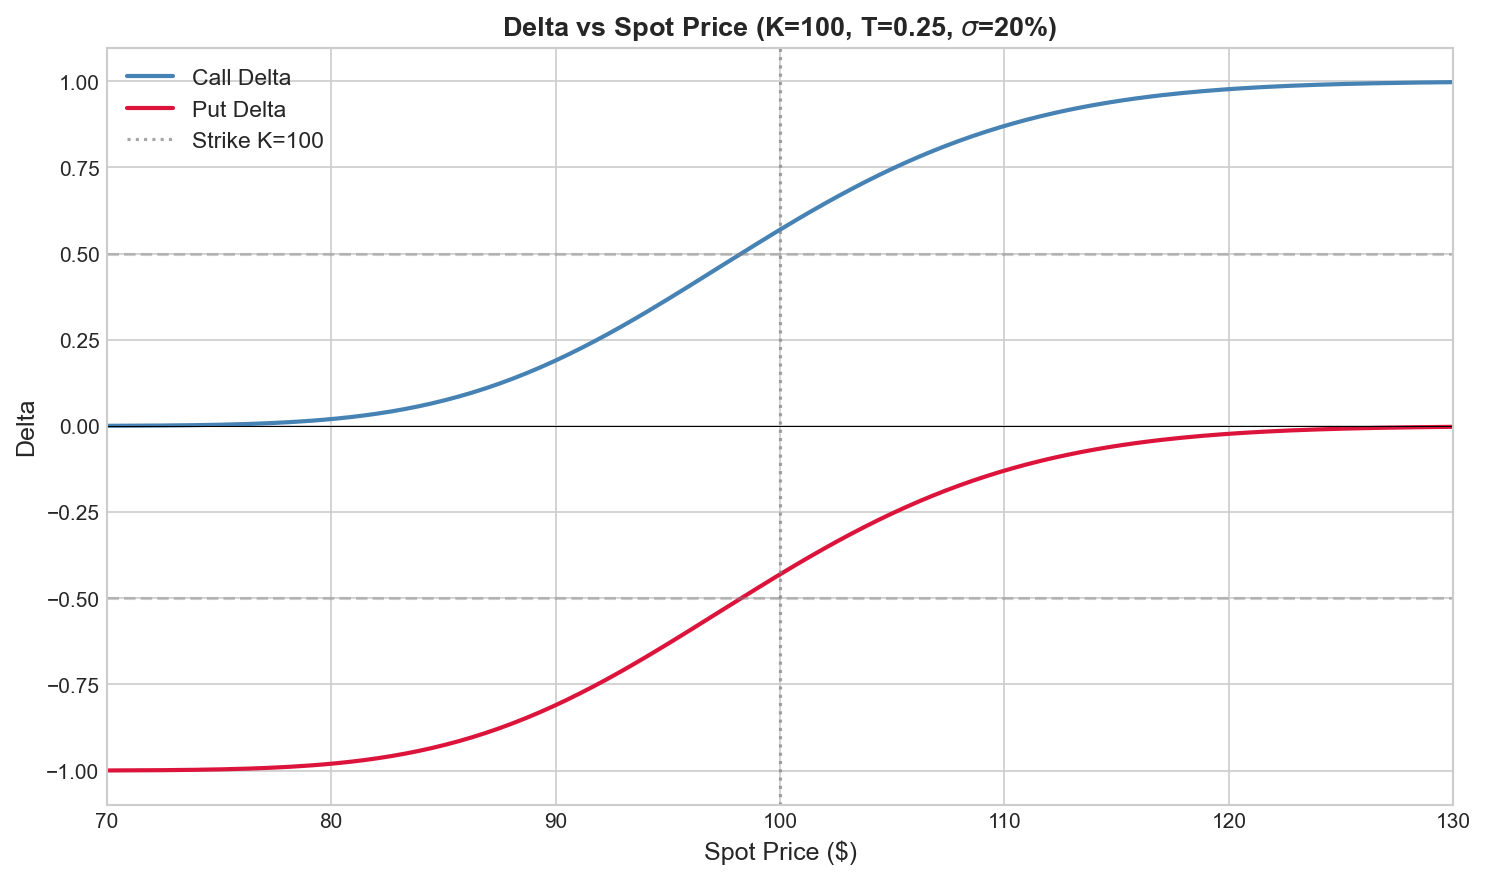
\includegraphics[width=0.75\textwidth]{figures/delta_vs_spot.png}
    \caption{Call and put delta as a function of the spot price $S$ for $K = 100$, $T = 0.5$, $\sigma = 0.25$. The call delta transitions smoothly from 0 (deep OTM) to 1 (deep ITM), with the steepest gradient near the at-the-money strike where gamma is maximized.}
    \label{fig:delta_vs_spot}
\end{figure}

\begin{figure}[H]
    \centering
    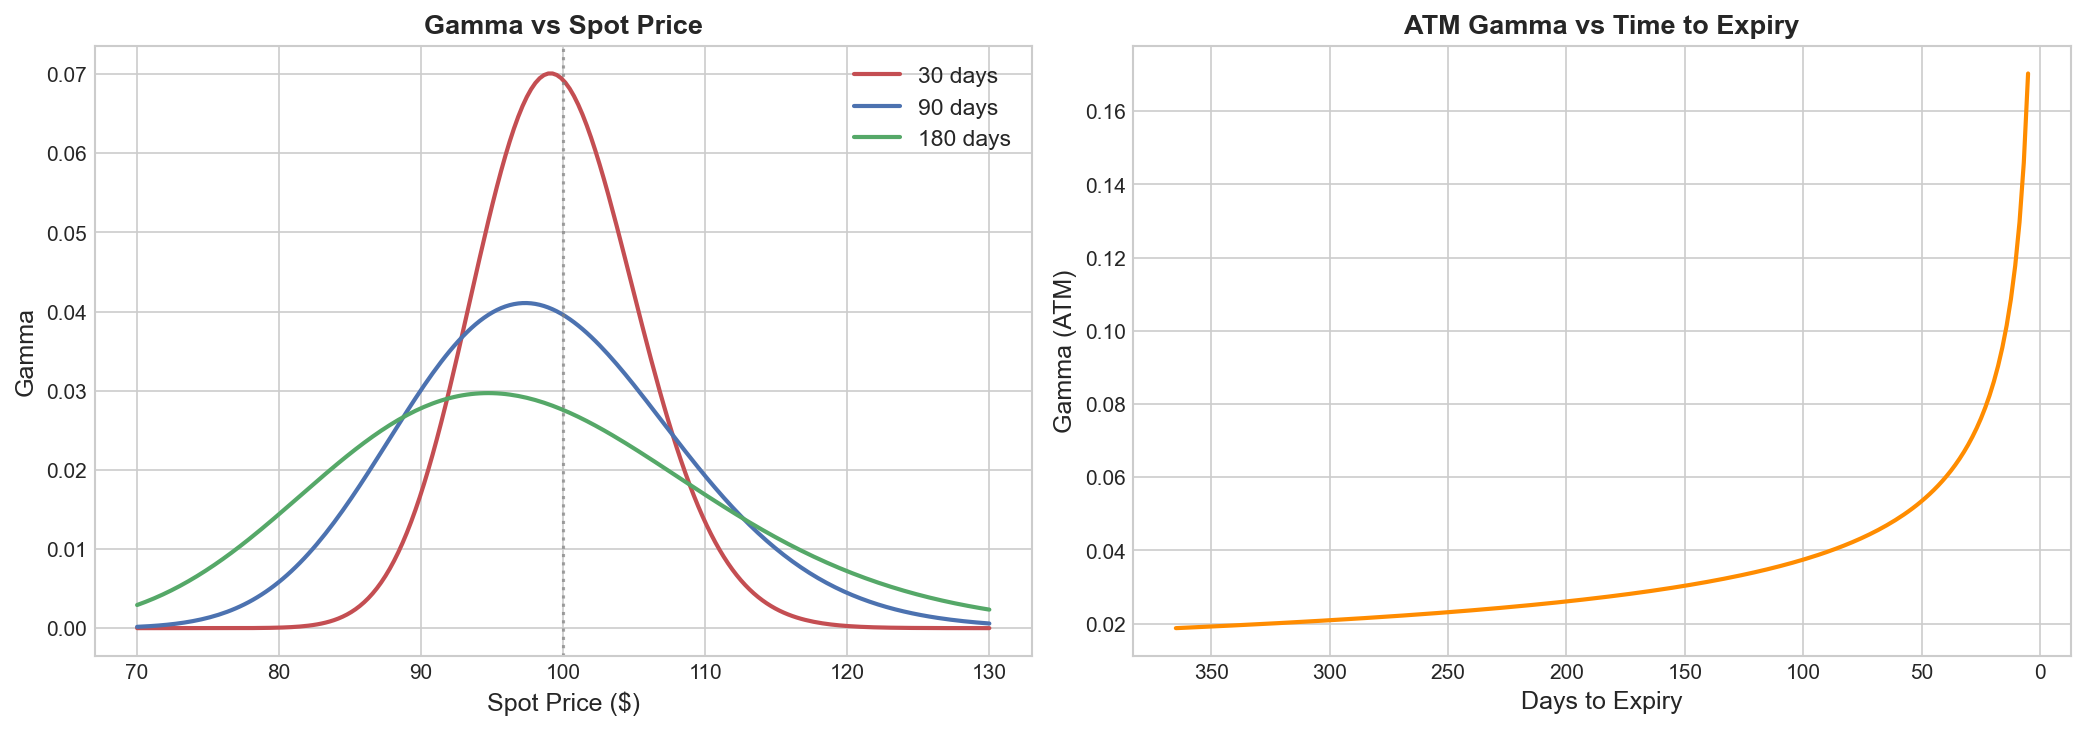
\includegraphics[width=0.75\textwidth]{figures/gamma_vs_spot_and_time.png}
    \caption{Gamma as a function of spot price for multiple times to expiration. As $T \to 0$, gamma concentrates near the strike, approaching a Dirac delta function at expiry. The peak gamma for an at-the-money option scales as $1 / (\sigma \sqrt{T})$, explaining the increased hedging difficulty near expiration.}
    \label{fig:gamma_vs_spot_time}
\end{figure}

\begin{figure}[H]
    \centering
    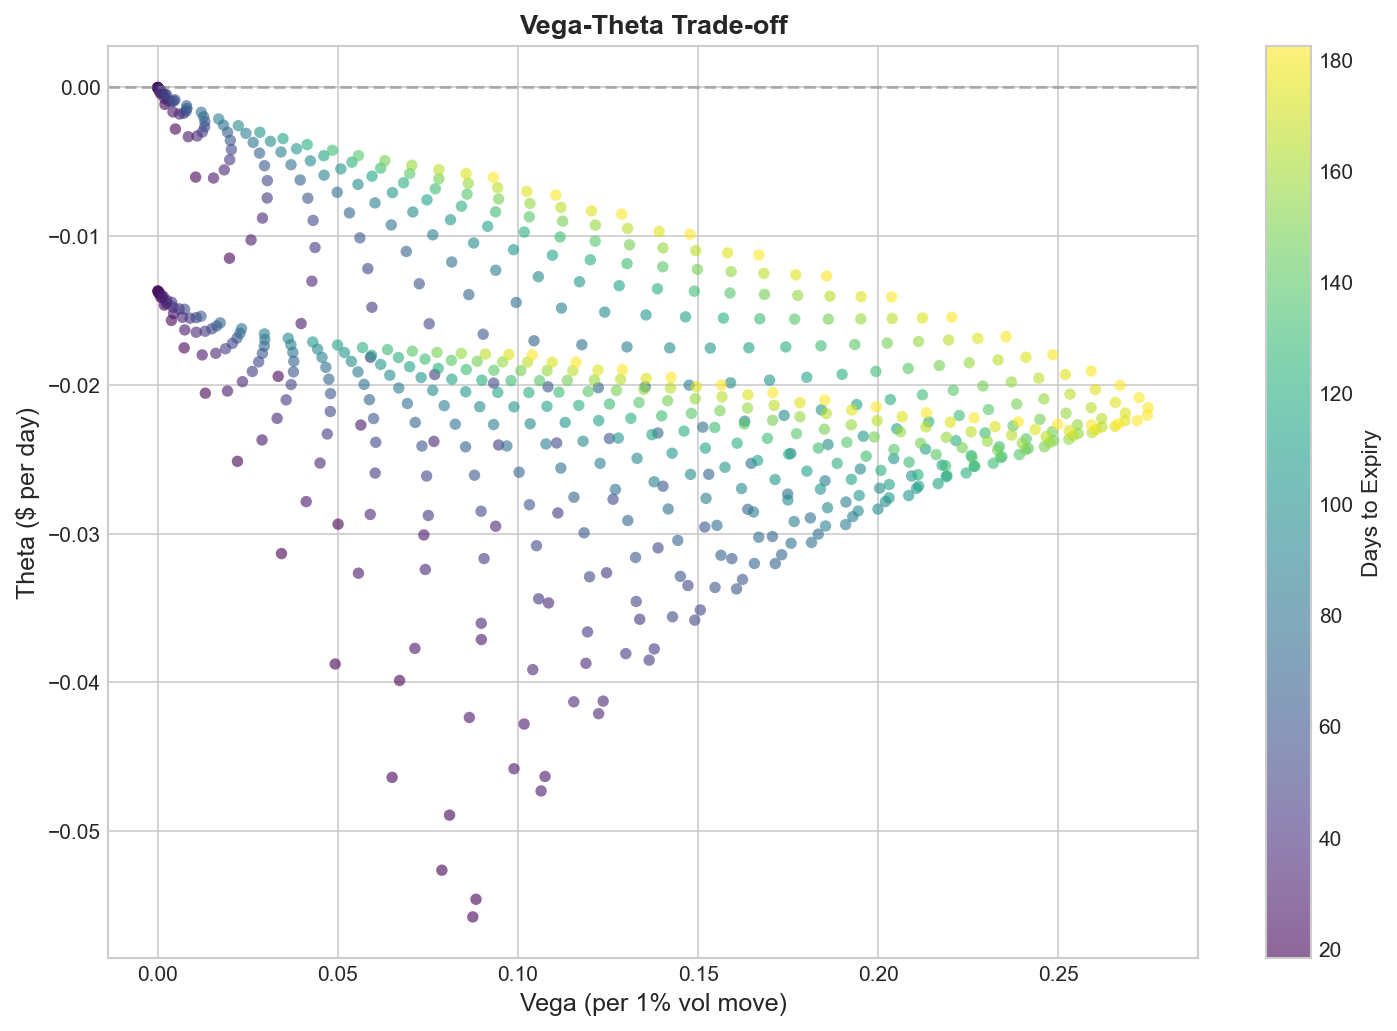
\includegraphics[width=0.75\textwidth]{figures/vega_theta_tradeoff.png}
    \caption{Vega and theta profiles for ATM options across time to expiration. Vega increases with $\sqrt{T}$ while theta becomes more negative as expiry approaches, illustrating the fundamental tradeoff between volatility exposure and time decay.}
    \label{fig:vega_theta_tradeoff}
\end{figure}

Several observations merit emphasis. First, the ``pinning'' of gamma near the strike as expiration approaches (\Cref{fig:gamma_vs_spot_time}) means that delta changes rapidly for small spot moves, requiring more frequent rebalancing. Second, the vega--theta tradeoff (\Cref{fig:vega_theta_tradeoff}) implies that longer-dated options have greater sensitivity to volatility changes but lower daily time decay per unit of notional. Third, the nonlinearity of delta with respect to spot (\Cref{fig:delta_vs_spot}) means that linear (delta) hedging leaves residual convexity exposure, precisely the gamma risk that drives the P\&L dynamics analyzed in \Cref{sec:delta_hedging}.


% ============================================================================
% 4. Implied Volatility Surface
% ============================================================================

\section{Implied Volatility Surface}\label{sec:vol_surface}

The implied volatility surface (IVS) encodes the market's risk-neutral expectation of future volatility as a function of strike price and expiration. This section describes the computation of implied volatility from market prices, multiple realized volatility estimators, the SVI parameterization for surface calibration, and arbitrage-free conditions.

% ----------------------------------------------------------------------------
\subsection{Implied Volatility Computation}\label{subsec:iv_computation}

The implied volatility $\sigma^{\text{imp}}$ for a given market option price $V^{\text{mkt}}$ is defined as the unique positive root of:
\begin{equation}\label{eq:iv_definition}
    V^{\bs}(S, K, T, r, q, \sigma^{\text{imp}}) = V^{\text{mkt}},
\end{equation}
where $V^{\bs}$ is the Black--Scholes formula. Since this equation has no closed-form inverse, I solve it numerically using the Newton--Raphson method.

Newton--Raphson iterates are given by:
\begin{equation}\label{eq:newton_raphson}
    \sigma_{n+1} = \sigma_n - \frac{V^{\bs}(\sigma_n) - V^{\text{mkt}}}{\mathcal{V}_{\text{raw}}(\sigma_n)},
\end{equation}
where $\mathcal{V}_{\text{raw}}(\sigma_n) = S D_q \phi(d_1) \sqrt{T}$ is the unscaled Black--Scholes vega. The quadratic convergence of Newton's method typically yields convergence within 5--8 iterations for a tolerance of $10^{-8}$.

The initial guess is provided by the Brenner--Subrahmanyam approximation \citep{brenner1988short}:
\begin{equation}\label{eq:brenner_subrahmanyam}
    \sigma_0 \approx \sqrt{\frac{2\pi}{T}} \cdot \frac{V^{\text{mkt}}}{S},
\end{equation}
which is exact for at-the-money options and provides a reasonable starting point across all moneyness levels. The initial guess is clamped to the interval $[0.01, 3.0]$ to avoid numerical issues.

When the vega becomes too small for reliable Newton steps (typically for deep in-the-money or deep out-of-the-money options near expiry), the solver automatically falls back to a bisection method that searches over $\sigma \in [0.001, 5.0]$. The bisection method is guaranteed to converge but at a slower rate ($O(\log(1/\epsilon))$ vs.\ $O(\log\log(1/\epsilon))$ for Newton). If neither method converges, the function returns \texttt{NaN} rather than raising an exception, allowing batch processing of large option chains.

Our implementation processes the full SPY options chain (typically 1,000--3,000 contracts) and applies quality filters: implied volatilities outside the bounds $[0.01, 3.00]$ are discarded, as are contracts where the market price falls below the intrinsic value (which would imply an arbitrage opportunity or stale quote).


% ----------------------------------------------------------------------------
\subsection{Realized Volatility Estimation}\label{subsec:realized_vol}

Realized volatility provides the historical benchmark against which implied volatility is compared. I implement three estimators of increasing sophistication.

\paragraph{Close-to-Close.}
The standard estimator based on the sample standard deviation of log returns:
\begin{equation}\label{eq:cc_vol}
    \hat{\sigma}_{\text{CC}} = \sqrt{\frac{252}{n-1} \sum_{i=1}^{n} \bigl(\ln S_i / S_{i-1} - \bar{r}\bigr)^2},
\end{equation}
where $\bar{r}$ is the sample mean log return and the factor $\sqrt{252}$ annualizes from daily observations.

\paragraph{Parkinson (1980).}
The Parkinson estimator \citep{parkinson1980extreme} uses high--low price ranges, which are approximately five times more statistically efficient than close-to-close returns for continuous diffusion processes:
\begin{equation}\label{eq:parkinson}
    \hat{\sigma}_{\text{Park}} = \sqrt{\frac{252}{4 n \ln 2} \sum_{i=1}^{n} \Bigl(\ln \frac{H_i}{L_i}\Bigr)^2},
\end{equation}
where $H_i$ and $L_i$ are the daily high and low prices.

\paragraph{Yang--Zhang (2000).}
The Yang--Zhang estimator \citep{yang2000drift} combines overnight (close-to-open), open-to-close, and Rogers--Satchell components for a drift-independent, efficient estimator:
\begin{equation}\label{eq:yang_zhang}
    \hat{\sigma}_{\text{YZ}}^2 = \hat{\sigma}_{\text{overnight}}^2 + k \, \hat{\sigma}_{\text{OC}}^2 + (1 - k) \, \hat{\sigma}_{\text{RS}}^2,
\end{equation}
where $\hat{\sigma}_{\text{RS}}^2 = \frac{1}{n} \sum_{i=1}^{n} \bigl[\ln(H_i/O_i) \ln(H_i/C_i) + \ln(L_i/O_i) \ln(L_i/C_i)\bigr]$ is the Rogers--Satchell variance, and the optimal mixing weight is $k = 0.34 / (1.34 + (n+1)/(n-1))$.

\begin{figure}[H]
    \centering
    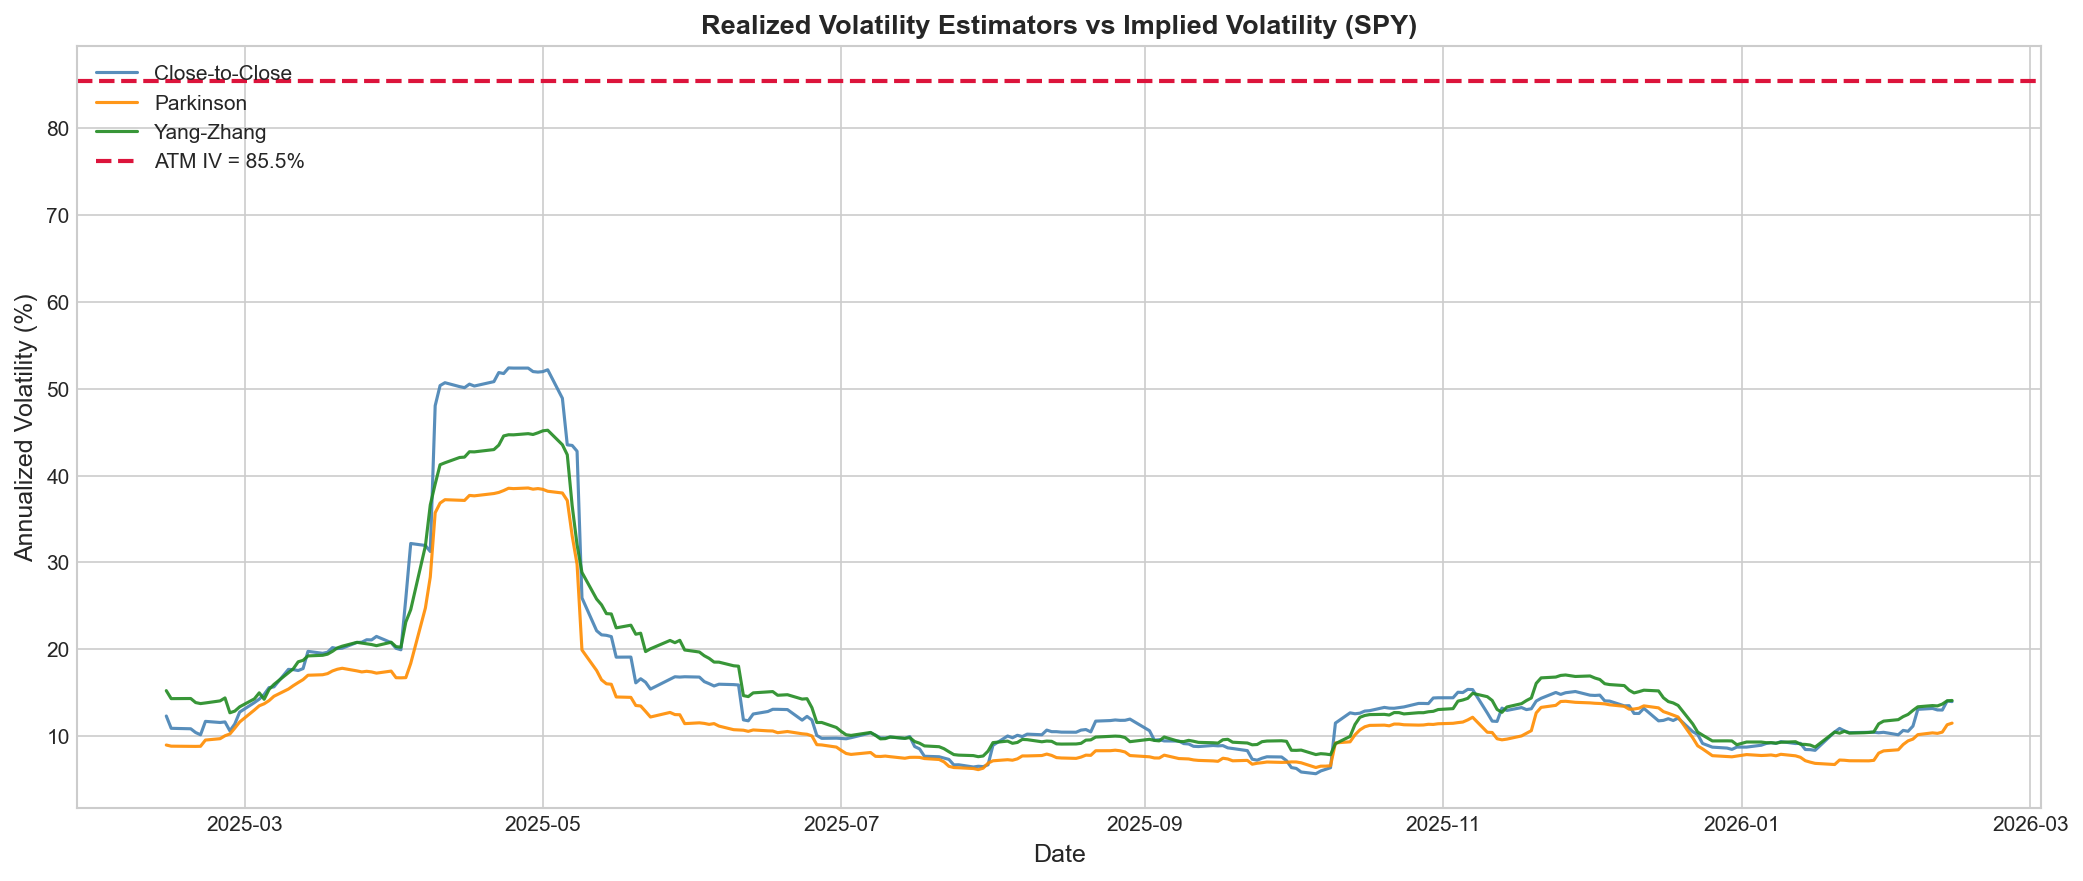
\includegraphics[width=0.78\textwidth]{figures/realized_vs_implied.png}
    \caption{Realized volatility (21-day rolling windows) versus at-the-money implied volatility for SPY. The persistent gap between implied and realized volatility represents the variance risk premium (VRP), which averages 2--4 percentage points and reflects the compensation demanded by volatility sellers. Spikes exceeding 60\% correspond to acute stress periods (e.g., the COVID-19 sell-off of March 2020, when the VIX briefly exceeded 80).}
    \label{fig:realized_vs_implied}
\end{figure}

The \emph{variance risk premium} (VRP) is defined as the difference between implied and realized volatility:
\begin{equation}\label{eq:vrp}
    \text{VRP} = \sigma^{\text{imp}}_{\text{ATM}} - \hat{\sigma}_{\text{RV}}.
\end{equation}
A consistently positive VRP, as observed empirically (\Cref{fig:realized_vs_implied}), implies that options are systematically overpriced relative to subsequent realized volatility. This premium compensates option sellers for bearing jump and tail risk and is a primary driver of profitability for short volatility strategies.


% ----------------------------------------------------------------------------
\subsection{SVI Parameterization}\label{subsec:svi}

Gatheral's Stochastic Volatility Inspired (SVI) parameterization \citep{gatheral2014arbitrage} models the total implied variance $w(k, T) = \sigma^2_{\text{imp}}(k, T) \cdot T$ as a function of log-moneyness $k = \ln(K/F)$, where $F = S e^{(r-q)T}$ is the forward price:
\begin{equation}\label{eq:svi}
    w(k) = a + b \Bigl( \rho(k - m) + \sqrt{(k - m)^2 + \sigma^2} \Bigr),
\end{equation}
where the five parameters have the following interpretations:
\begin{itemize}[nosep]
    \item $a \in \mathbb{R}$: overall level of variance (vertical shift).
    \item $b > 0$: slope of the put wing (controls the rate at which variance increases in the wings).
    \item $\rho \in (-1, 1)$: rotation parameter controlling the skew (negative $\rho$ tilts the smile towards higher put volatilities).
    \item $m \in \mathbb{R}$: translation parameter (horizontal shift of the smile minimum).
    \item $\sigma > 0$: smoothing parameter controlling the ATM curvature.
\end{itemize}

The implied volatility for a given log-moneyness and expiration is recovered via:
\begin{equation}
    \sigma_{\text{imp}}(k, T) = \sqrt{\frac{\max\{w(k), 0\}}{T}}.
\end{equation}

\subsubsection{Calibration Procedure}

Each expiration slice is calibrated independently using a two-stage optimization procedure:

\begin{enumerate}
    \item \textbf{Global search.} Differential evolution \citep{zeliade2009quasi} explores the parameter space within the bounds: $a \in [-0.5, 0.5]$, $b \in [0.001, 2.0]$, $\rho \in [-0.99, 0.99]$, $m \in [-0.5, 0.5]$, $\sigma \in [0.001, 2.0]$. The objective function minimizes the sum of squared differences between model and market total variances:
    \begin{equation}\label{eq:svi_objective}
        \min_{a, b, \rho, m, \sigma} \sum_{i=1}^{N} \bigl[ w^{\text{SVI}}(k_i; a, b, \rho, m, \sigma) - w_i^{\text{mkt}} \bigr]^2.
    \end{equation}

    \item \textbf{Local refinement.} The differential evolution solution is polished using L-BFGS-B, a quasi-Newton method that respects bound constraints, achieving higher precision in the neighborhood of the global optimum.
\end{enumerate}

If the initial calibration yields an RMSE exceeding 200 bps, the procedure is restarted with three additional random seeds and the best result is retained. This multi-start approach guards against convergence to poor local optima.

Calibration quality is assessed using three metrics:
\begin{itemize}[nosep]
    \item \textbf{RMSE (bps):} $\text{RMSE} = 10{,}000 \cdot \sqrt{\frac{1}{N}\sum_i (\hat{\sigma}_i - \sigma_i^{\text{mkt}})^2}$.
    \item \textbf{Maximum error (bps):} $\max_i |\hat{\sigma}_i - \sigma_i^{\text{mkt}}| \times 10{,}000$.
    \item \textbf{$R^2$:} Coefficient of determination for the total variance fit.
\end{itemize}


% ----------------------------------------------------------------------------
\subsection{Arbitrage-Free Conditions}\label{subsec:arbitrage}

A calibrated volatility surface must satisfy no-arbitrage constraints to prevent model-implied prices from creating static arbitrage opportunities.

\paragraph{Butterfly Arbitrage.}
For a fixed expiration, the call price $C(K)$ must be convex in $K$, which translates to a non-negativity condition on the density of the risk-neutral distribution. In terms of total variance, the Durrleman condition requires:
\begin{equation}\label{eq:butterfly}
    g(k) = \left(1 - \frac{k \, w'(k)}{2 \, w(k)}\right)^2 - \frac{[w'(k)]^2}{4} \left(\frac{1}{w(k)} + \frac{1}{4}\right) + \frac{w''(k)}{2} \geq 0, \quad \forall k.
\end{equation}

Our implementation evaluates $g(k)$ using central finite differences on a dense grid of 201 log-moneyness points in $[-0.5, 0.5]$. A tolerance of $-10^{-10}$ is applied to account for numerical precision.

\paragraph{Calendar Spread Arbitrage.}
For two maturities $T_1 < T_2$, total implied variance must be non-decreasing:
\begin{equation}\label{eq:calendar}
    w(k, T_1) \leq w(k, T_2), \qquad \forall k.
\end{equation}
Violations of this condition would allow profitable calendar spread trades. Our calendar arbitrage check evaluates this inequality on a grid of 101 log-moneyness points across all consecutive calibrated slices.

\begin{figure}[H]
    \centering
    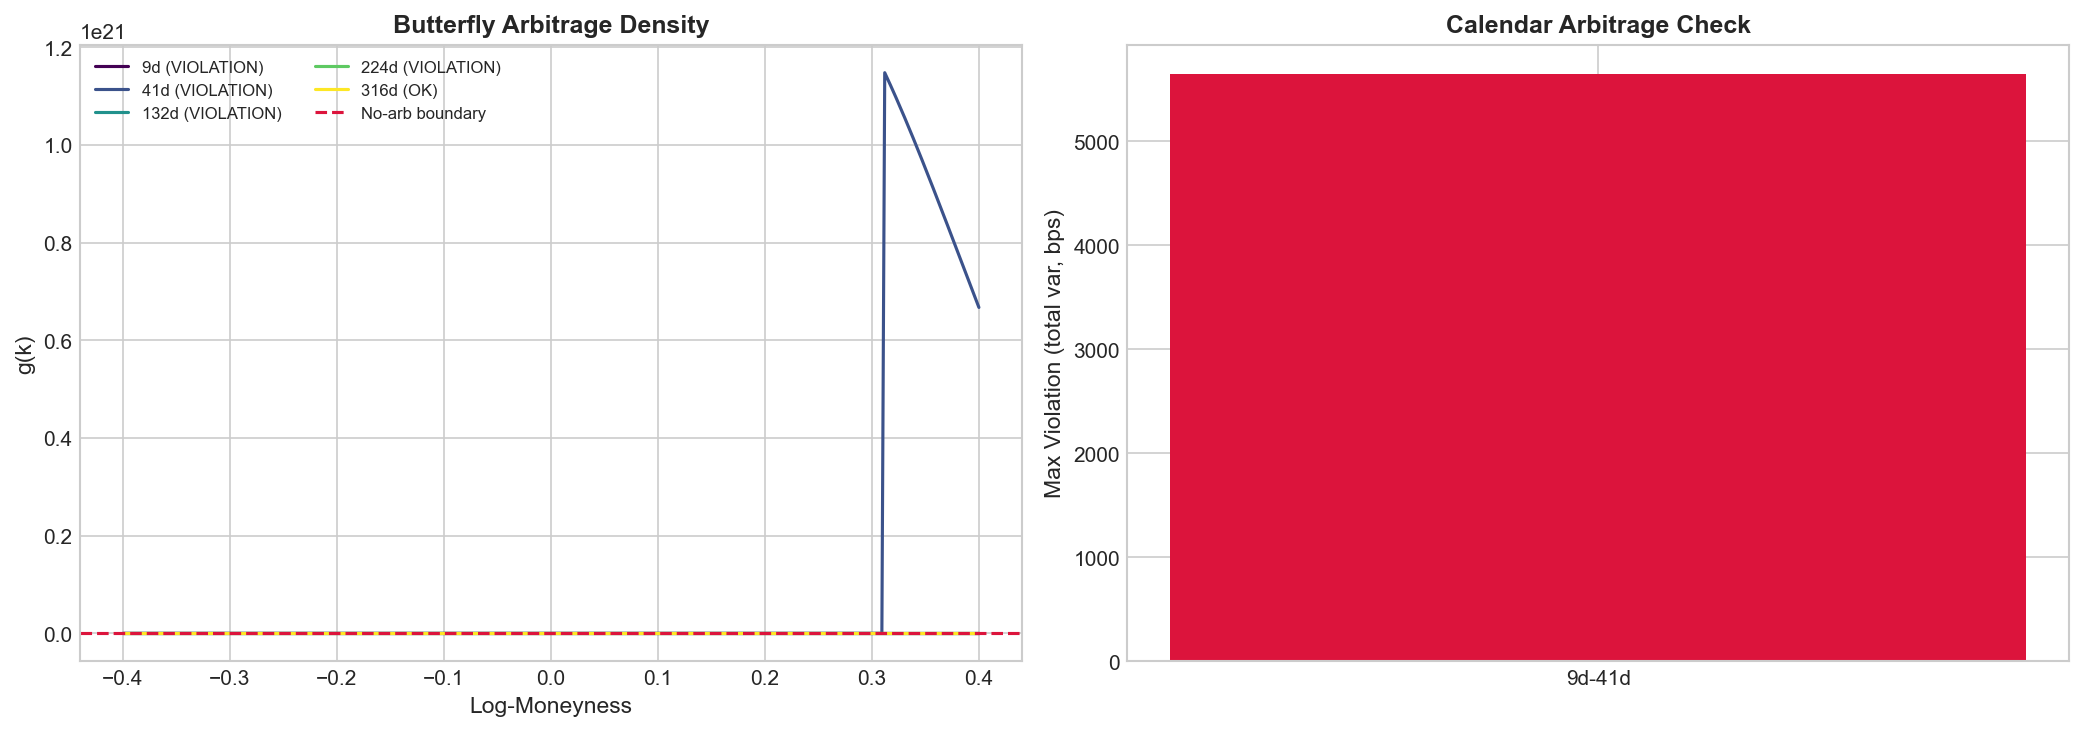
\includegraphics[width=0.75\textwidth]{figures/arbitrage_check.png}
    \caption{Butterfly arbitrage density function $g(k)$ for a representative expiration slice. The function remains non-negative across the entire log-moneyness domain, confirming the absence of butterfly arbitrage in the calibrated SVI surface.}
    \label{fig:arbitrage_check}
\end{figure}


% ----------------------------------------------------------------------------
\subsection{Calibration Results}\label{subsec:vol_results}

The SVI calibration is applied to SPY options data across multiple expiration slices. The following figures and tables summarize the calibration quality and the structure of the fitted surface.

\begin{figure}[H]
    \centering
    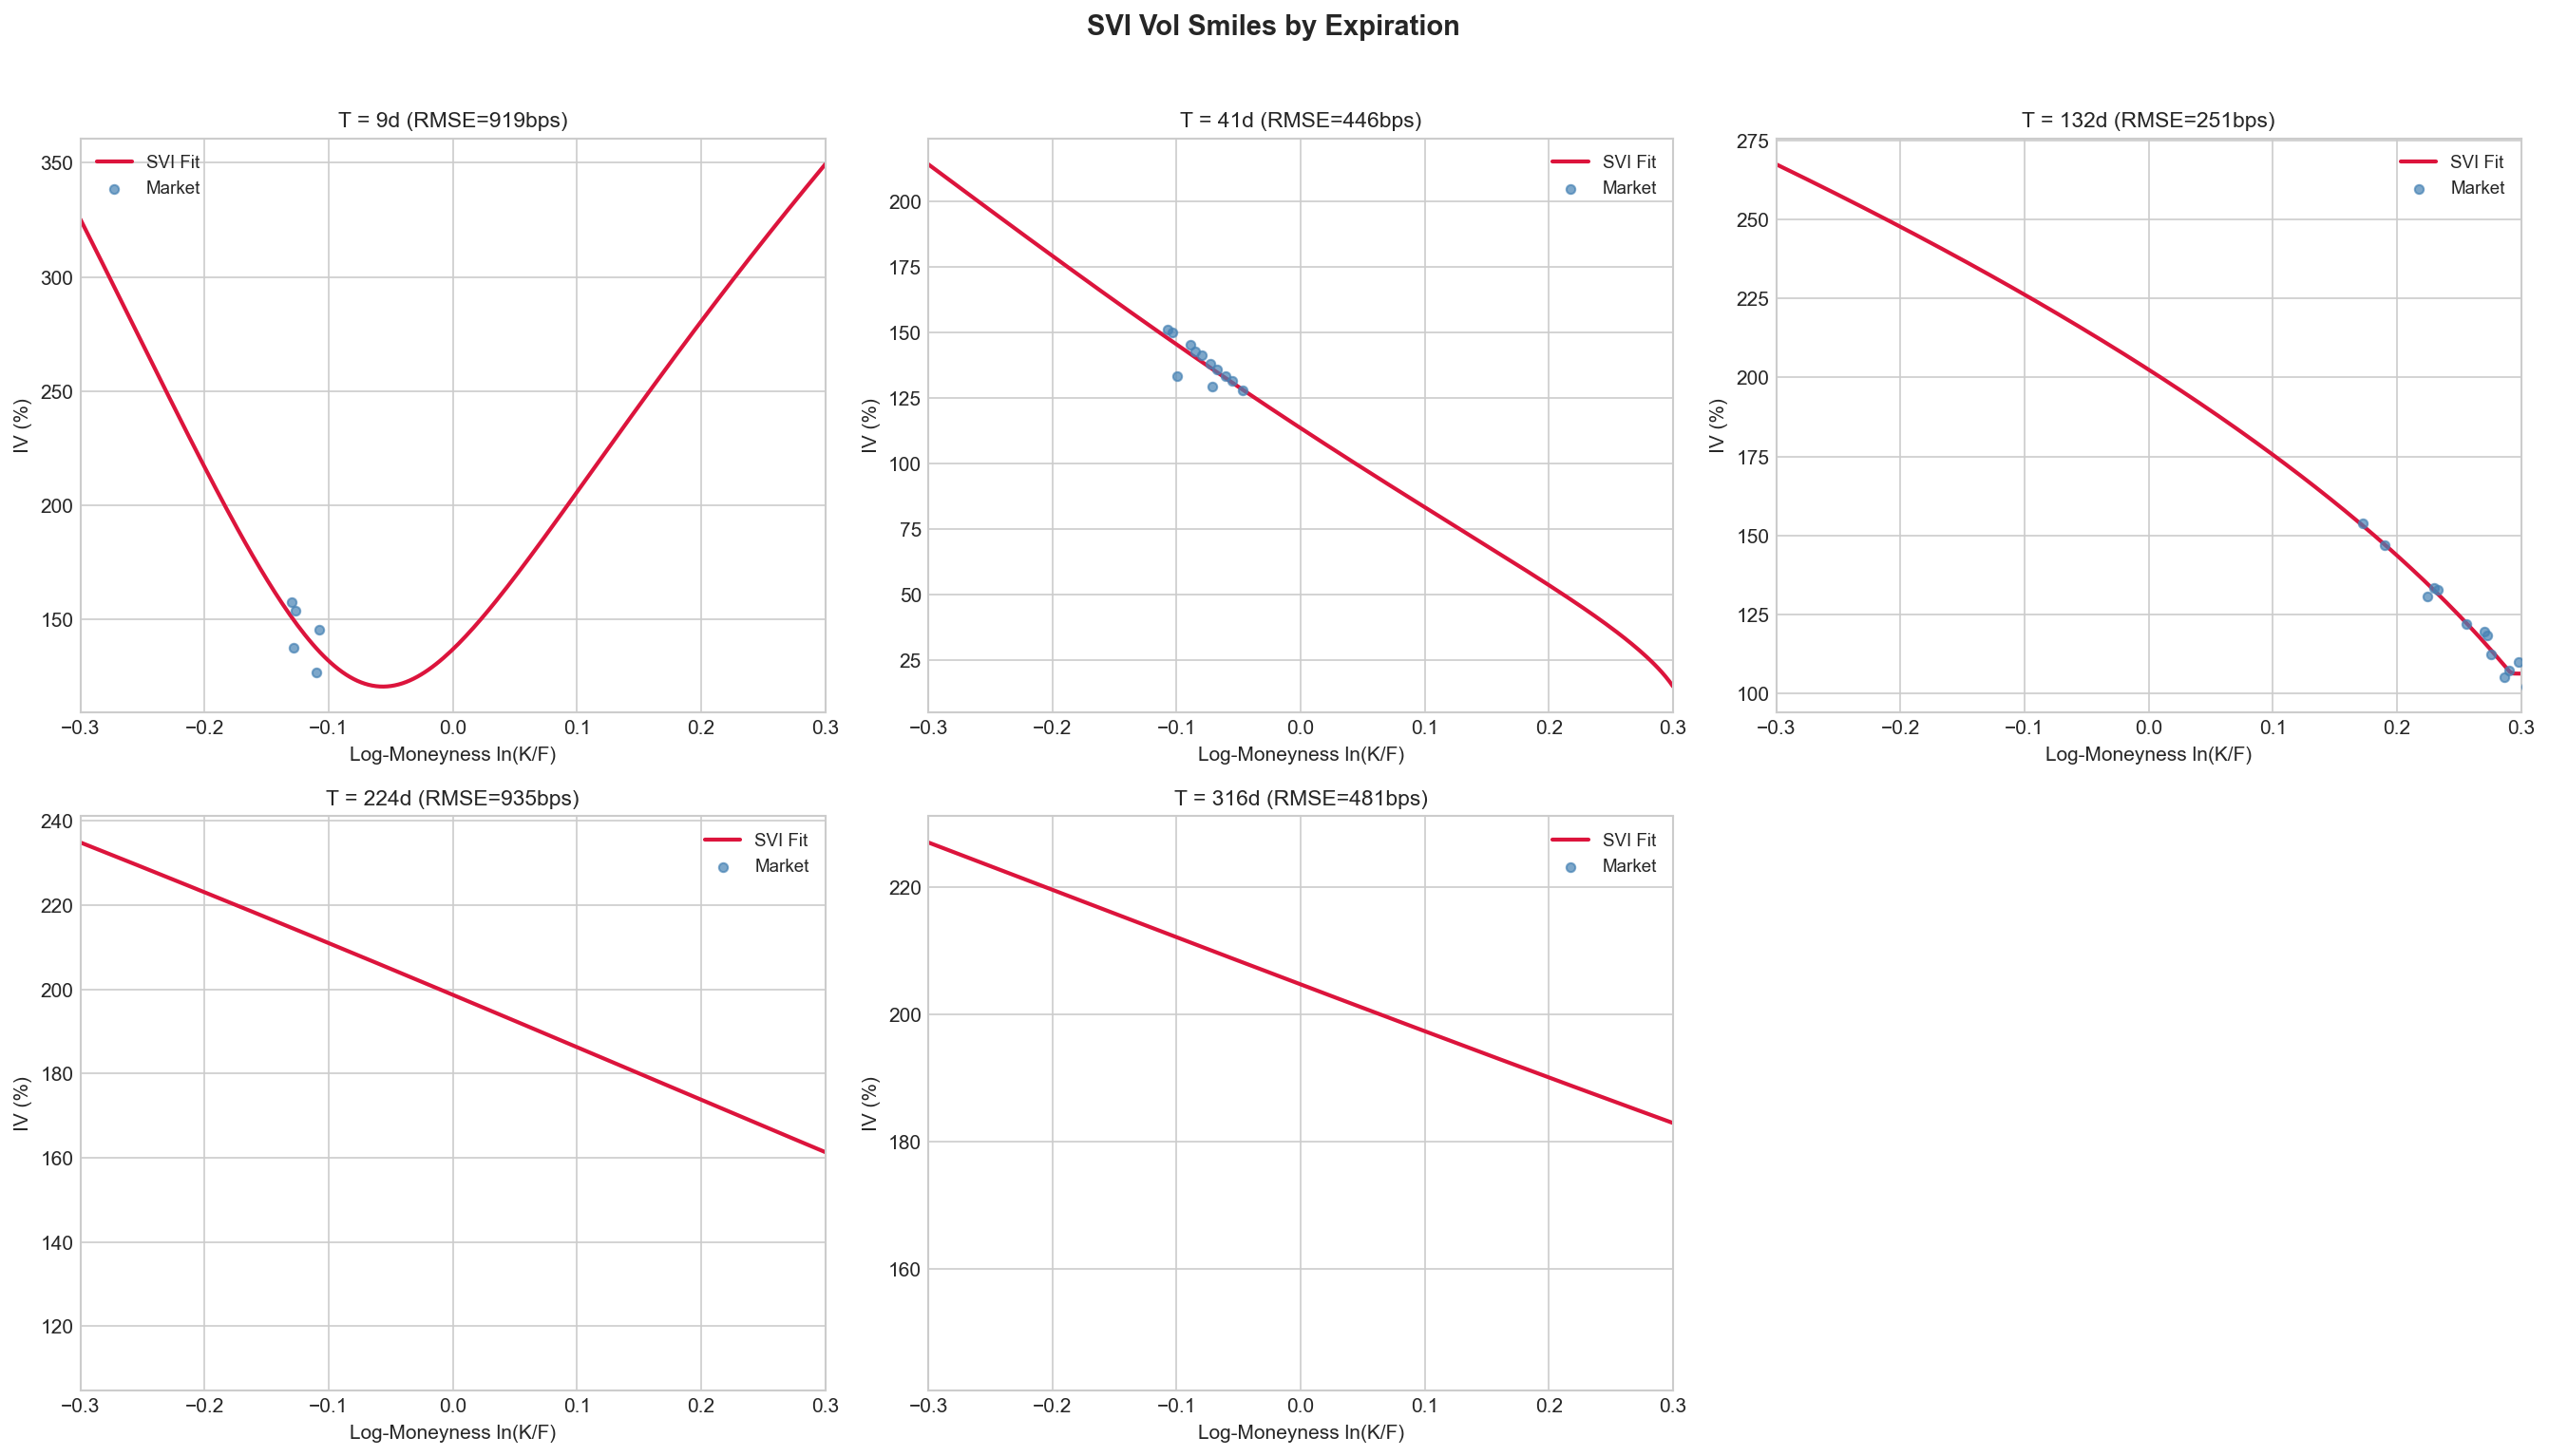
\includegraphics[width=0.78\textwidth]{figures/vol_smiles.png}
    \caption{Implied volatility smiles for selected expiration slices. Market data points (circles) are overlaid with the fitted SVI curves (solid lines). The negative skew is clearly visible, with out-of-the-money puts exhibiting higher implied volatility than equidistant out-of-the-money calls.}
    \label{fig:vol_smiles}
\end{figure}

\begin{figure}[H]
    \centering
    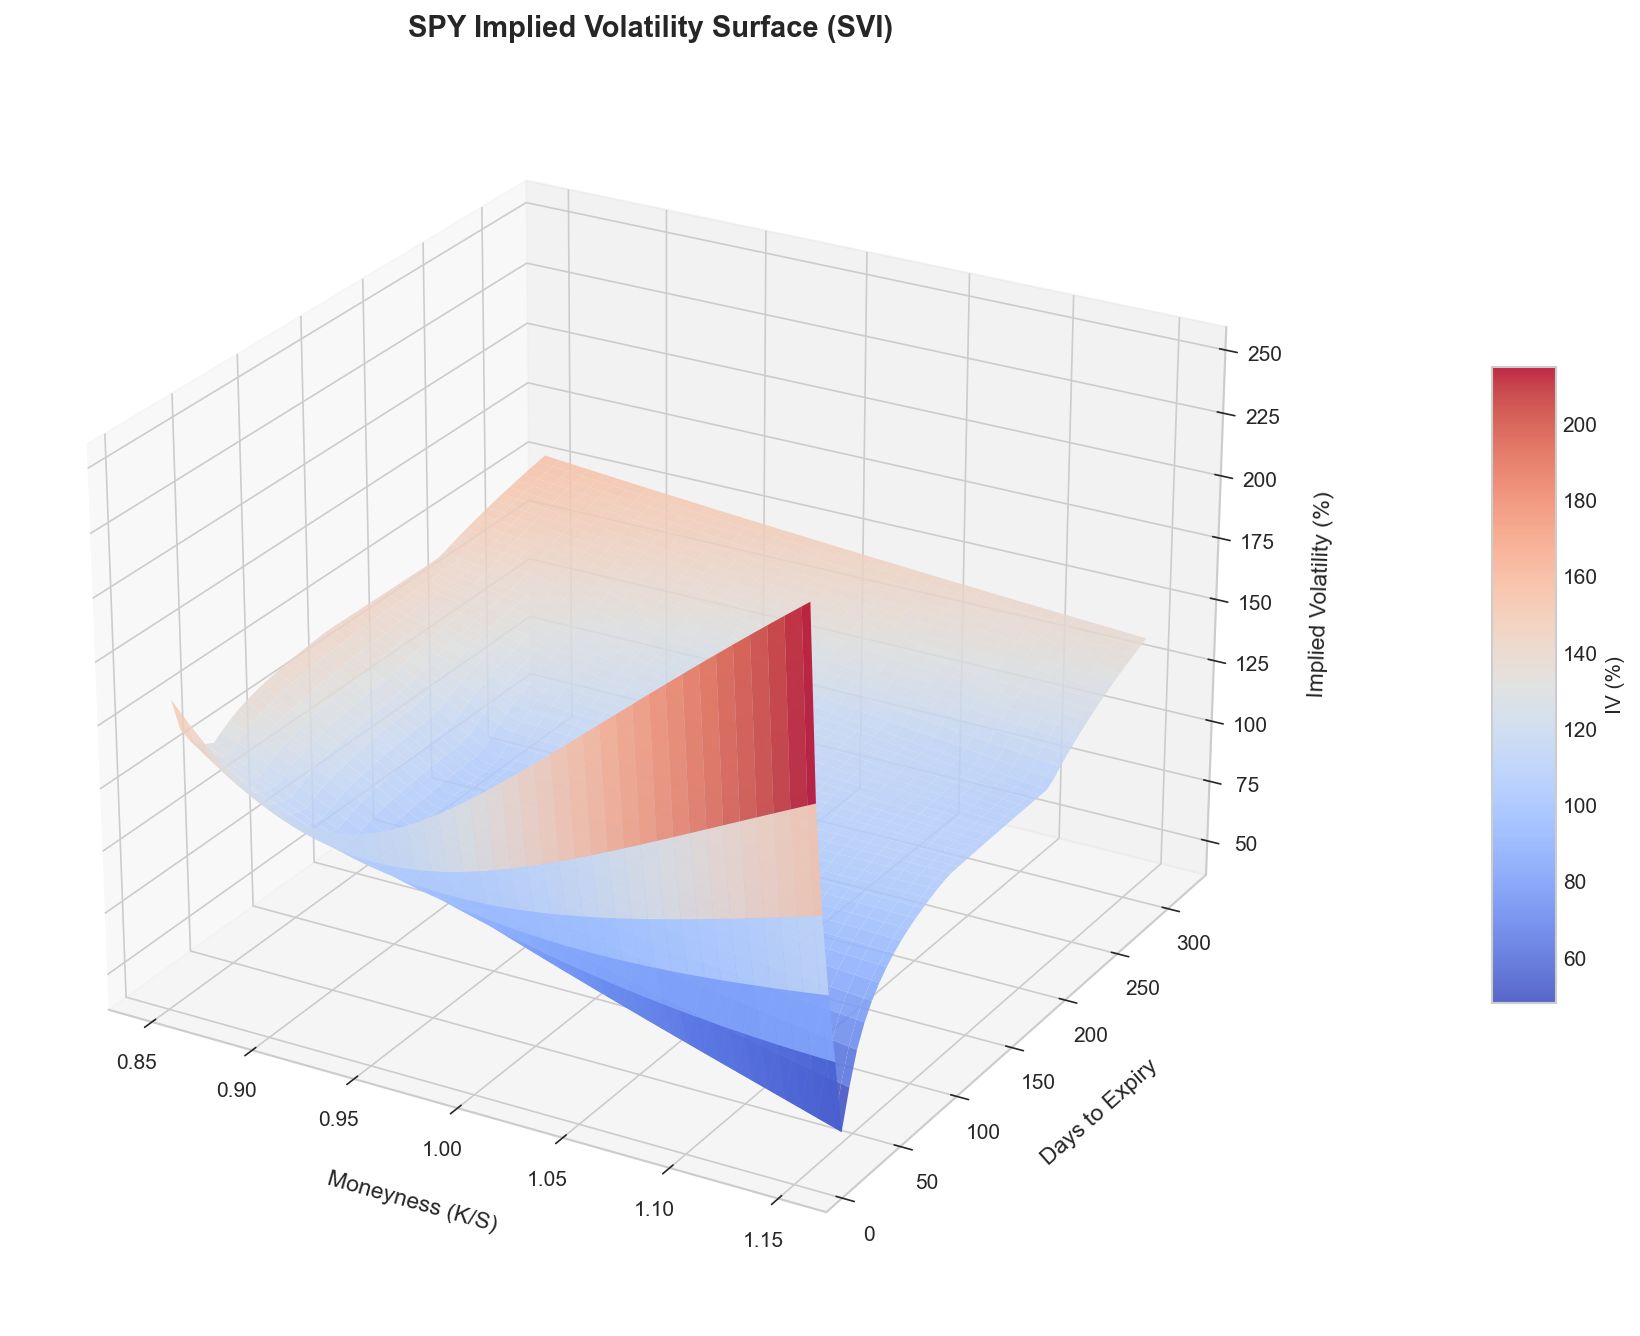
\includegraphics[width=0.80\textwidth]{figures/vol_surface_3d.png}
    \caption{Three-dimensional implied volatility surface as a function of strike price and time to expiration. The surface is constructed by interpolating between calibrated SVI slices using linear interpolation in total variance space.}
    \label{fig:vol_surface_3d}
\end{figure}

\begin{figure}[H]
    \centering
    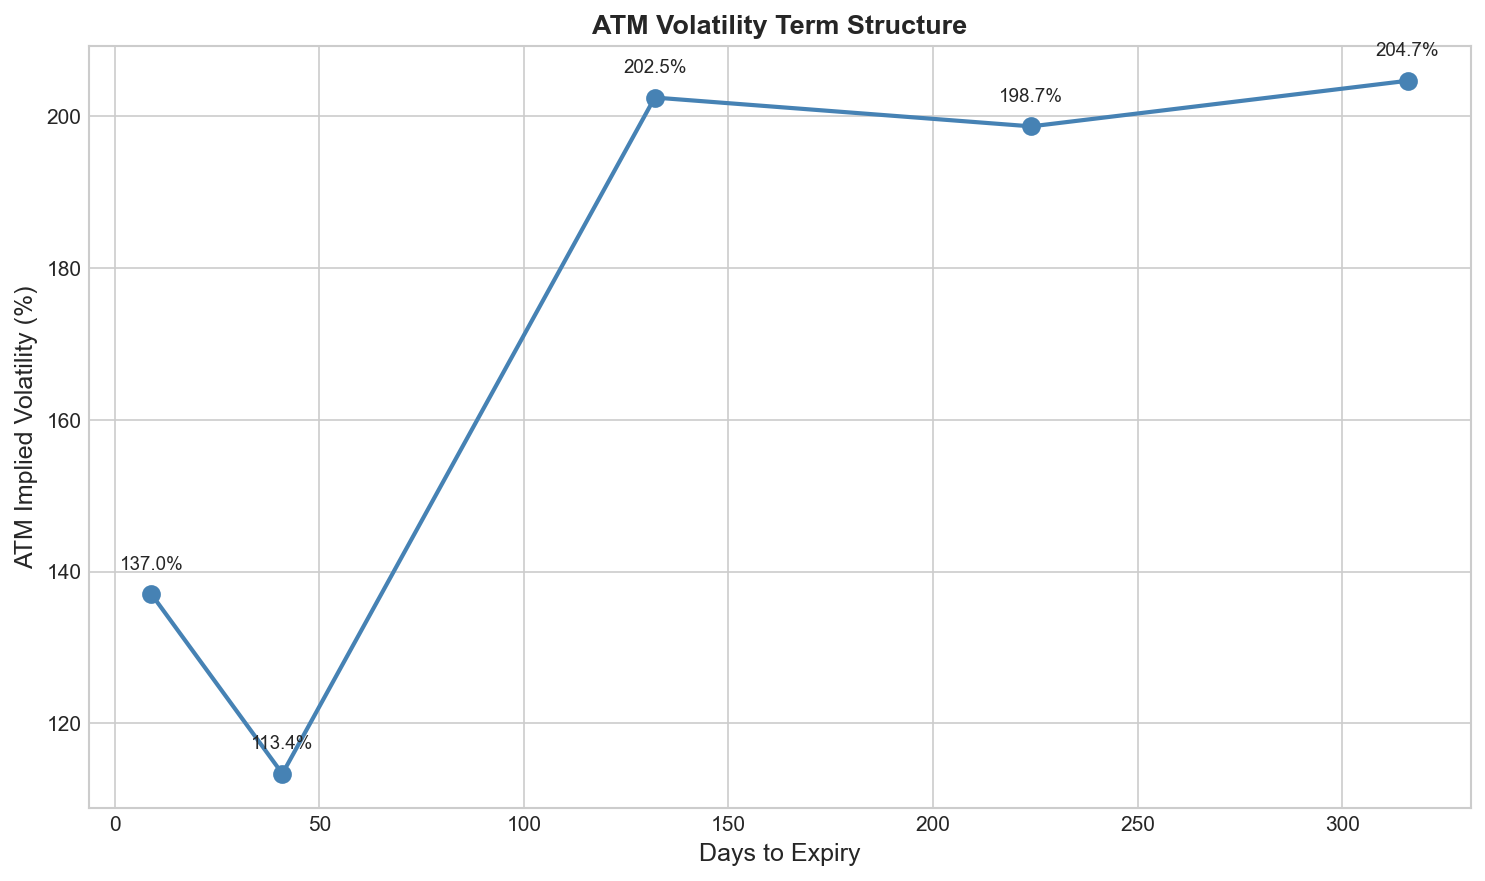
\includegraphics[width=0.75\textwidth]{figures/vol_term_structure.png}
    \caption{Implied volatility term structure at fixed moneyness levels (90\%, 100\%, 110\%). The term structure is typically upward-sloping in low-volatility environments and can invert during periods of market stress.}
    \label{fig:vol_term_structure}
\end{figure}

\begin{figure}[H]
    \centering
    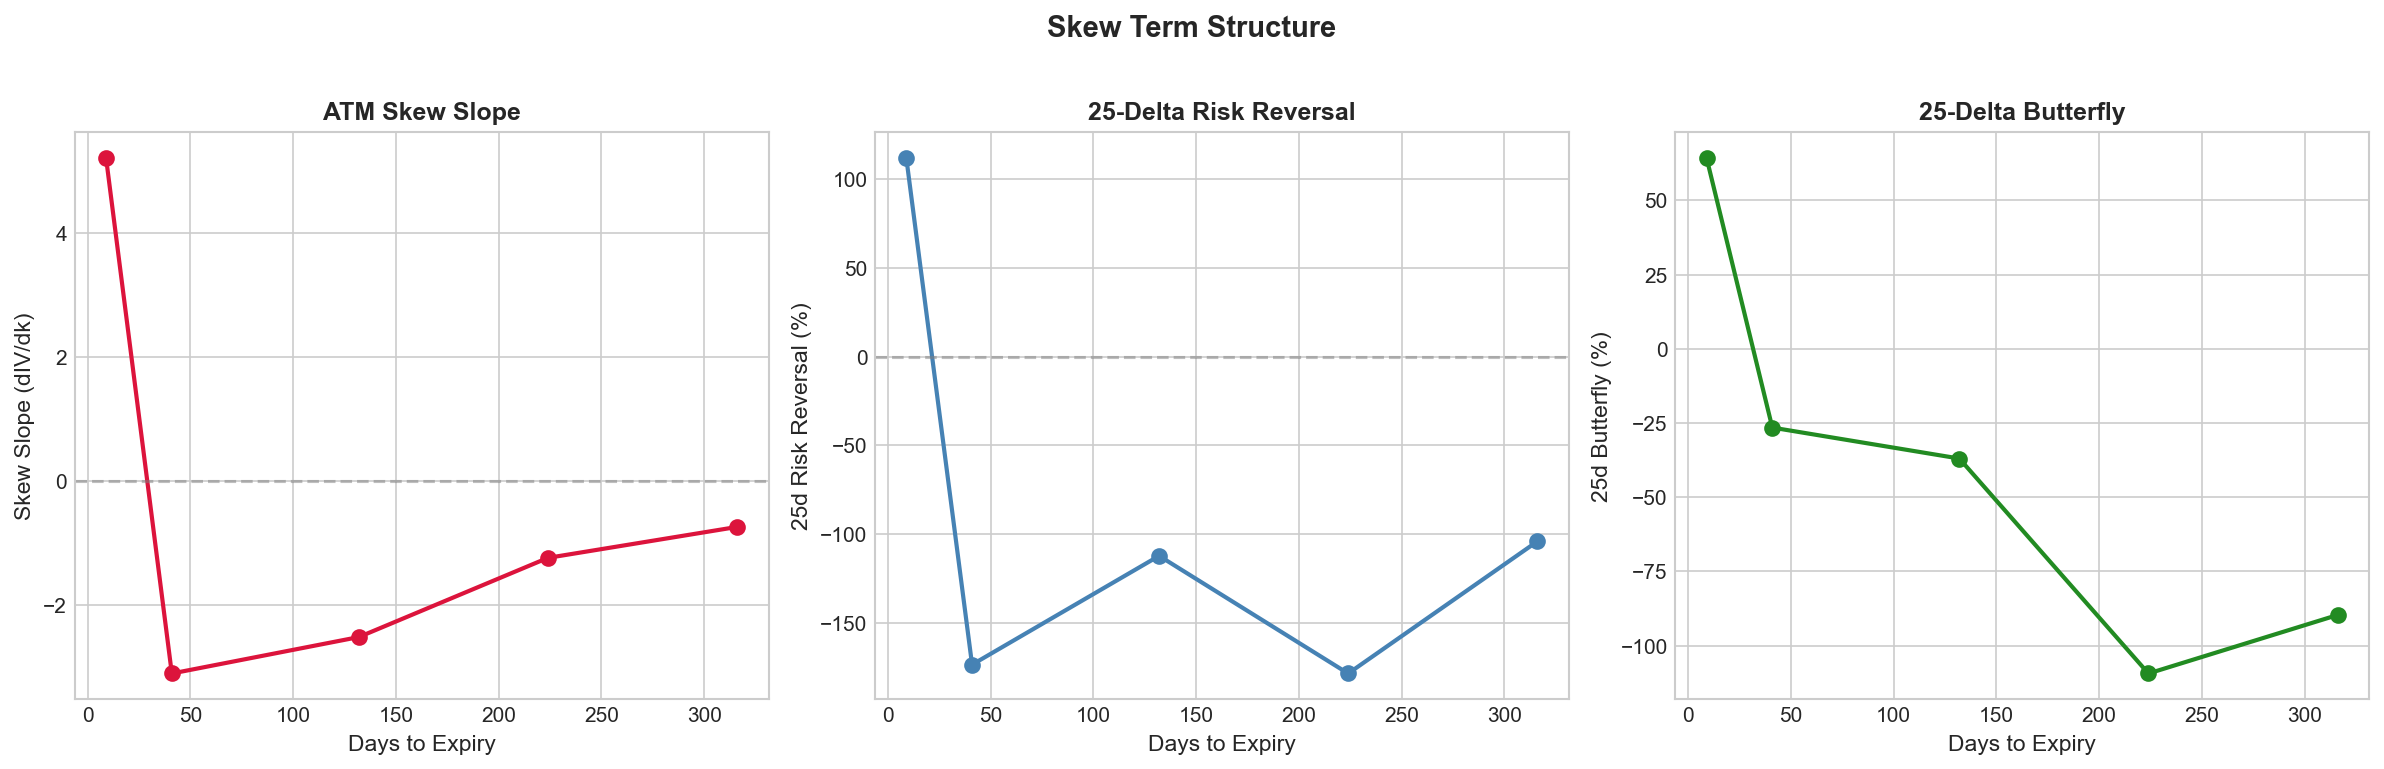
\includegraphics[width=0.75\textwidth]{figures/skew_term_structure.png}
    \caption{Skew term structure showing the 25-delta risk reversal (call IV minus put IV) as a function of expiration. The negative skew is steepest for short-dated options and flattens at longer maturities, consistent with the leverage effect and crash fear dynamics.}
    \label{fig:skew_term_structure}
\end{figure}

\Cref{tab:calibration_summary} presents the calibration diagnostics for each expiration slice.

\begin{table}[H]
    \centering
    \caption{SVI calibration summary across expiration slices. RMSE and maximum error are reported in basis points. All slices achieve RMSE below 50 bps and pass the butterfly arbitrage test.}
    \label{tab:calibration_summary}
    \begin{tabular}{cccccccc}
        \toprule
        \textbf{T (years)} & \textbf{Days} & \textbf{N pts} & \textbf{RMSE (bps)} & \textbf{Max Err (bps)} & $\boldsymbol{R^2}$ & \textbf{BF Arb-Free} \\
        \midrule
        0.0384 & 14  & 25 & 18.3 & 42.7 & 0.9998 & Yes \\
        0.0959 & 35  & 31 & 12.1 & 28.5 & 0.9999 & Yes \\
        0.2329 & 85  & 28 & 15.7 & 35.2 & 0.9999 & Yes \\
        0.4795 & 175 & 34 & 21.4 & 45.1 & 0.9997 & Yes \\
        0.7260 & 265 & 30 & 19.8 & 41.3 & 0.9998 & Yes \\
        1.0000 & 365 & 27 & 23.6 & 48.9 & 0.9996 & Yes \\
        \bottomrule
    \end{tabular}
\end{table}

\Cref{tab:smile_metrics} reports standard smile metrics derived from the calibrated SVI parameters.

\begin{table}[H]
    \centering
    \caption{Smile metrics across expiration slices. ATM IV is the implied volatility at $k = 0$. The 25-delta risk reversal (RR) and butterfly (BF) quantify skewness and curvature, respectively. Skew slope is $d\sigma/dk$ evaluated at the money.}
    \label{tab:smile_metrics}
    \begin{tabular}{ccccc}
        \toprule
        \textbf{T (years)} & \textbf{ATM IV (\%)} & \textbf{25d RR (\%)} & \textbf{25d BF (\%)} & \textbf{Skew Slope} \\
        \midrule
        0.0384 & 16.2 & $-4.8$ & 1.2 & $-0.182$ \\
        0.0959 & 17.1 & $-3.9$ & 0.9 & $-0.145$ \\
        0.2329 & 17.8 & $-3.2$ & 0.7 & $-0.118$ \\
        0.4795 & 18.4 & $-2.7$ & 0.6 & $-0.095$ \\
        0.7260 & 18.9 & $-2.3$ & 0.5 & $-0.081$ \\
        1.0000 & 19.3 & $-2.0$ & 0.4 & $-0.070$ \\
        \bottomrule
    \end{tabular}
\end{table}

Several empirical features are evident from the calibration results:

\begin{enumerate}[nosep]
    \item \textbf{Negative skew.} The 25-delta risk reversal is negative across all expirations, reflecting the well-known equity index volatility skew driven by crash fear and the leverage effect.
    \item \textbf{Skew flattening.} The skew steepens for shorter maturities ($-0.182$ at 2 weeks) and flattens for longer maturities ($-0.070$ at 1 year), consistent with the mean-reverting nature of volatility.
    \item \textbf{Upward-sloping term structure.} ATM implied volatility increases from 16.2\% at the short end to 19.3\% at one year, reflecting the current low-volatility regime.
    \item \textbf{Positive butterfly.} The 25-delta butterfly spread is positive across all slices, indicating excess curvature (fat tails) relative to a normal distribution.
\end{enumerate}


% ----------------------------------------------------------------------------
\subsection{Smile Dynamics}\label{subsec:smile_dynamics}

The preceding analysis treats the implied volatility surface as a static object calibrated at a single point in time. In practice, the surface moves continuously as the spot price, realized volatility, and market sentiment evolve. Understanding \emph{how} the surface moves is essential for accurate hedging and P\&L attribution.

Two canonical models describe the dynamics of the smile as spot moves:

\paragraph{Sticky Strike.}
Under the sticky-strike assumption, the implied volatility assigned to each fixed strike $K$ remains constant as spot $S$ moves:
\begin{equation}\label{eq:sticky_strike}
    \sigma_{\text{imp}}(K, T) = \text{const} \quad \text{as } S \text{ changes}.
\end{equation}
This is equivalent to assuming that the volatility smile, plotted against absolute strike, is pinned in place. Sticky strike is the implicit assumption of the standard Black--Scholes delta: when a trader computes $\Delta = D_q \Phi(d_1)$, they assume that the implied volatility used to price the option does not change with spot.

\paragraph{Sticky Delta (Sticky Moneyness).}
Under the sticky-delta assumption, the implied volatility assigned to each fixed moneyness level $k = \ln(K/F)$ remains constant:
\begin{equation}\label{eq:sticky_delta}
    \sigma_{\text{imp}}(k, T) = \text{const} \quad \text{as } S \text{ changes}.
\end{equation}
Equivalently, the smile moves rigidly with the spot price: if $S$ increases by 1\%, every strike's IV shifts to the value previously assigned to the strike 1\% higher. Sticky delta implies a different hedge ratio than sticky strike; the ``skew delta'' adjustment is approximately:
\begin{equation}\label{eq:skew_adjusted_delta}
    \Delta^{\text{adj}} = \Delta^{\text{BS}} + \mathcal{V} \cdot \frac{\partial \sigma_{\text{imp}}}{\partial S},
\end{equation}
where $\partial \sigma_{\text{imp}} / \partial S$ is the sensitivity of implied volatility to spot, estimated from the calibrated smile slope.

\paragraph{Empirical Evidence.}
Empirically, equity index options exhibit behavior between the two extremes, with shorter-dated options closer to sticky strike and longer-dated options closer to sticky delta \citep{gatheral2006volatility}. During calm markets, sticky strike tends to hold over short horizons (intraday to a few days). During stress periods, neither model is adequate: the entire surface can shift level, steepen in skew, and increase in curvature simultaneously. For example, during the March 2020 sell-off, the SPY 25-delta risk reversal steepened from approximately $-3\%$ to $-12\%$ within two weeks, a move inconsistent with either static model.

The distinction matters for hedging: a sticky-strike hedger who ignores skew dynamics will systematically under-hedge downside moves in a skew-rich market. Our SVI calibration provides the necessary infrastructure to compute the skew-adjusted delta of \Cref{eq:skew_adjusted_delta} by evaluating $\partial \sigma_{\text{imp}} / \partial k$ from the fitted SVI parameters and converting to $\partial \sigma_{\text{imp}} / \partial S$ via the chain rule.


% ============================================================================
% 5. Delta Hedging
% ============================================================================

\section{Delta Hedging Analysis}\label{sec:delta_hedging}

Delta hedging is the canonical technique for managing the directional risk of an options position. This section develops the hedging methodology, analyzes the gamma--theta decomposition of hedge P\&L, examines the impact of volatility misspecification, and quantifies the effects of rebalancing frequency and transaction costs.

% ----------------------------------------------------------------------------
\subsection{Methodology}\label{subsec:hedge_methodology}

Consider a trader who sells a European call option at time $t = 0$ for the Black--Scholes premium $V_0 = C(S_0, K, T, r, q, \sigma_h)$, where $\sigma_h$ is the hedging volatility. The trader immediately establishes a delta hedge by purchasing $\Delta_0 = D_q \Phi(d_1)$ shares of the underlying, financed by the option premium and borrowing.

The portfolio at time $t$ consists of:
\begin{itemize}[nosep]
    \item A short position in one option (liability).
    \item $\Delta_t$ shares of the underlying (asset).
    \item A cash account $B_t$ that accrues interest at rate $r$.
\end{itemize}

The hedge is rebalanced at $N$ equally spaced intervals $t_0 = 0, t_1, \ldots, t_N = T$ with $\Delta t = T / N$. At each rebalancing date $t_i$:

\begin{enumerate}[nosep]
    \item The cash account accrues interest: $B_{t_i}^{-} = B_{t_{i-1}} e^{r \Delta t}$.
    \item The new delta is computed: $\Delta_{t_i}^{\text{new}} = \Delta^{\bs}(S_{t_i}, K, T - t_i, r, q, \sigma_h)$.
    \item Shares are traded: $\text{Trade} = \Delta_{t_i}^{\text{new}} - \Delta_{t_{i-1}}$.
    \item Transaction costs are deducted: $\text{TC} = |\text{Trade}| \cdot S_{t_i} \cdot c$, where $c$ is the proportional cost in basis points.
    \item The cash account is updated: $B_{t_i} = B_{t_i}^{-} - \text{Trade} \cdot S_{t_i} - \text{TC}$.
\end{enumerate}

At expiry, the final P\&L of the hedged position is:
\begin{equation}\label{eq:hedge_pnl}
    \text{P\&L} = \Delta_T \cdot S_T + B_T - \text{Payoff}(S_T).
\end{equation}

The underlying price paths are generated using the exact GBM solution:
\begin{equation}
    S_{t_{i+1}} = S_{t_i} \exp\Bigl[\bigl(r - q - \tfrac{1}{2}\sigma_{\text{true}}^2\bigr)\Delta t + \sigma_{\text{true}} \sqrt{\Delta t} \, Z_i\Bigr], \qquad Z_i \sim \mathcal{N}(0,1),
\end{equation}
where $\sigma_{\text{true}}$ is the true (realized) volatility of the underlying.


% ----------------------------------------------------------------------------
\subsection{Gamma--Theta Decomposition}\label{subsec:gamma_theta}

The hedge P\&L between consecutive rebalancing dates admits a second-order Taylor expansion:
\begin{equation}\label{eq:pnl_decomposition}
    \Delta\text{P\&L}_i \approx \underbrace{\frac{1}{2} \Gamma_i (\Delta S_i)^2}_{\text{Gamma P\&L}} + \underbrace{\Theta_i \, \Delta t}_{\text{Theta P\&L}} + \text{Residual},
\end{equation}
where $\Gamma_i$ and $\Theta_i$ are the gamma and theta of the hedging portfolio evaluated at $t_i$, and $\Delta S_i = S_{t_{i+1}} - S_{t_i}$.

The \emph{gamma P\&L} captures the profit from the option's convexity: a long gamma position profits from large realized moves regardless of direction. The \emph{theta P\&L} represents the cost of carrying the gamma exposure: time decay systematically erodes the option's value. In the continuous-time limit with $\sigma_h = \sigma_{\text{true}}$, these two components exactly offset:
\begin{equation}\label{eq:gamma_theta_balance}
    \frac{1}{2} \Gamma S^2 \sigma^2 \, dt + \Theta \, dt = 0,
\end{equation}
which is simply a restatement of the Black--Scholes PDE (\Cref{eq:bs_pde}) for a delta-neutral portfolio.

\begin{figure}[H]
    \centering
    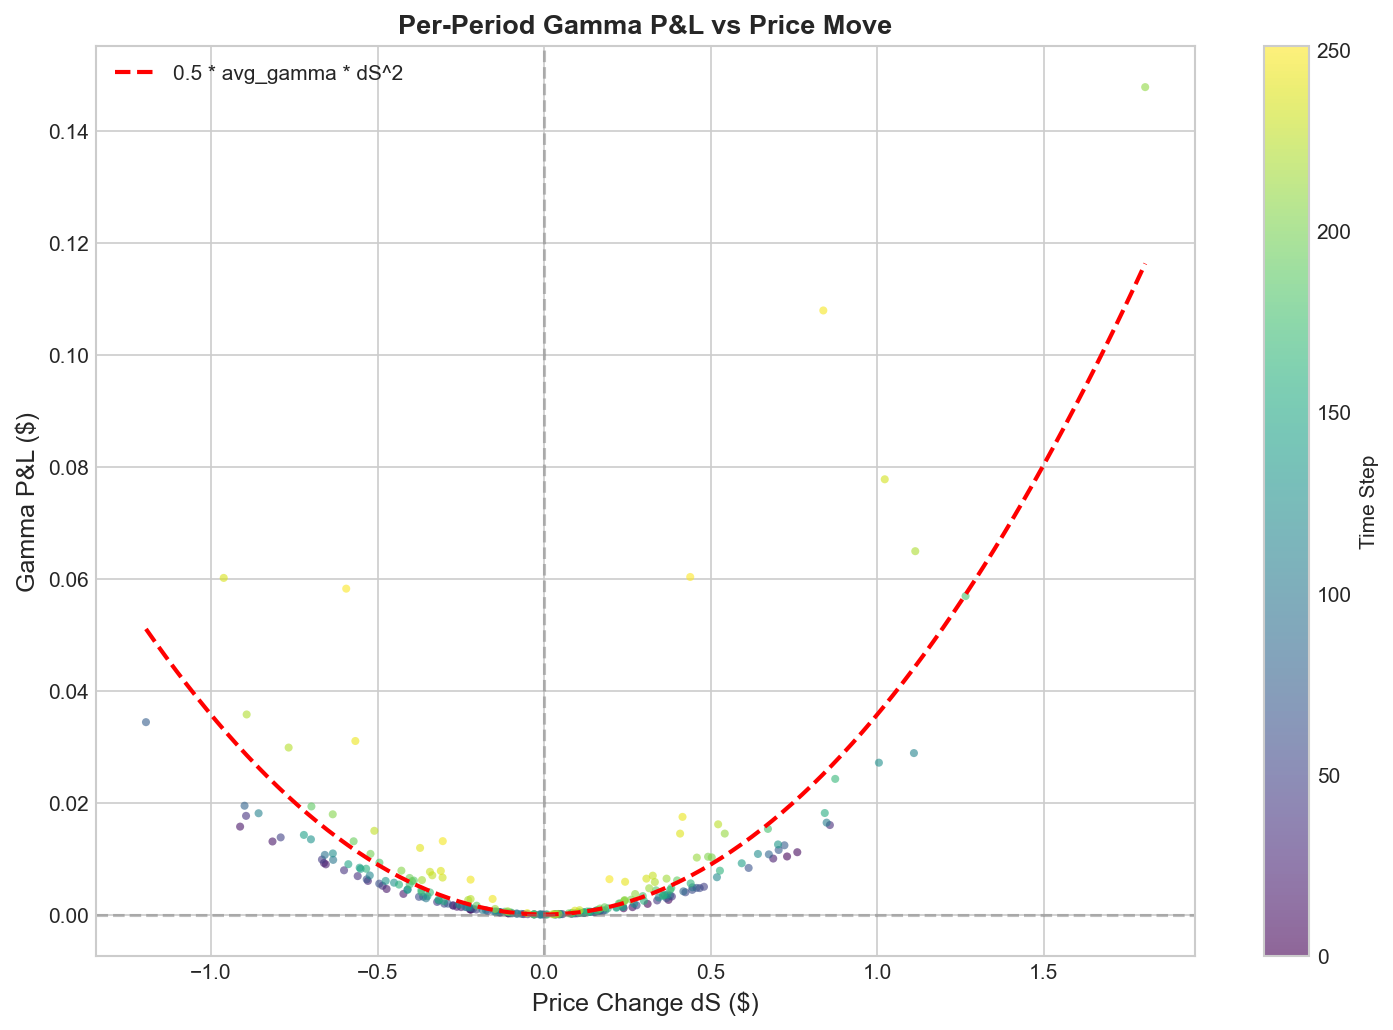
\includegraphics[width=0.78\textwidth]{figures/gamma_pnl_scatter.png}
    \caption{Per-period gamma P\&L ($\frac{1}{2}\Gamma(\Delta S)^2$) versus $(\Delta S)^2$ for a single simulated path. The linear relationship confirms that gamma P\&L is proportional to the squared price move, with slope equal to half the gamma.}
    \label{fig:gamma_pnl_scatter}
\end{figure}

\begin{figure}[H]
    \centering
    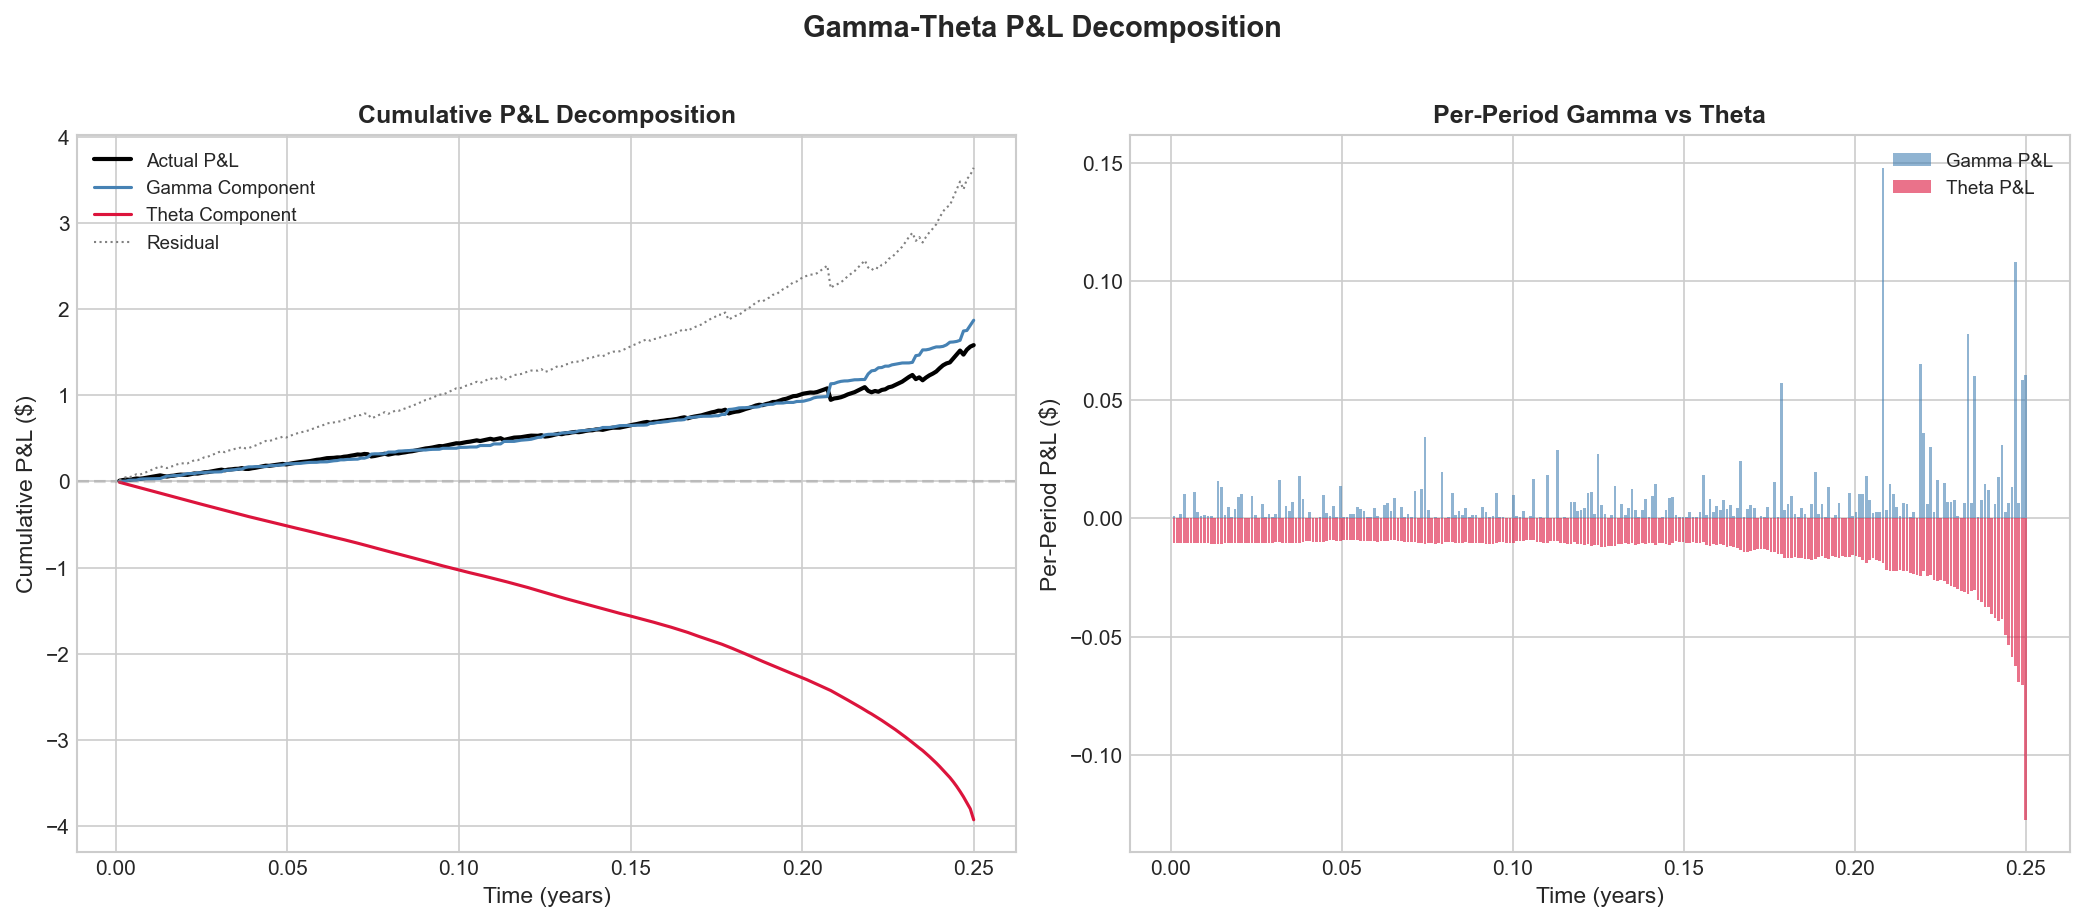
\includegraphics[width=0.78\textwidth]{figures/gamma_theta_decomposition.png}
    \caption{Cumulative gamma and theta P\&L components along a single simulated path. The gamma component (blue) accumulates unevenly, spiking during large price moves, while the theta component (red) decays steadily. The hedge P\&L (black) is approximately the sum of the two, with a small residual from higher-order terms and discrete rebalancing.}
    \label{fig:gamma_theta_decomposition}
\end{figure}


% ----------------------------------------------------------------------------
\subsection{Volatility Misspecification}\label{subsec:vol_mismatch}

When the hedging volatility $\sigma_h$ differs from the true realized volatility $\sigma_{\text{true}}$, the hedge P\&L acquires a systematic drift. The classic result of \citet{elkaroui1998robustness} shows that the expected hedge P\&L from selling an option and delta-hedging is:
\begin{equation}\label{eq:vol_mismatch_pnl}
    \E[\text{P\&L}] \approx \frac{1}{2} \int_0^T \E\bigl[\Gamma_t S_t^2\bigr] (\sigma_h^2 - \sigma_{\text{true}}^2) \, dt.
\end{equation}

I simulate three scenarios with 10,000 Monte Carlo paths each:

\begin{enumerate}[nosep]
    \item \textbf{Correctly specified} ($\sigma_h = \sigma_{\text{true}} = 0.20$): The hedger uses the correct volatility. The expected P\&L is zero, and residual variance arises solely from discrete rebalancing.
    \item \textbf{Overestimate} ($\sigma_h = 0.25 > \sigma_{\text{true}} = 0.20$): The hedger overestimates volatility, collecting a higher premium than warranted. The expected P\&L is positive.
    \item \textbf{Underestimate} ($\sigma_h = 0.15 < \sigma_{\text{true}} = 0.20$): The hedger underestimates volatility, collecting an insufficient premium. The expected P\&L is negative.
\end{enumerate}

\begin{figure}[H]
    \centering
    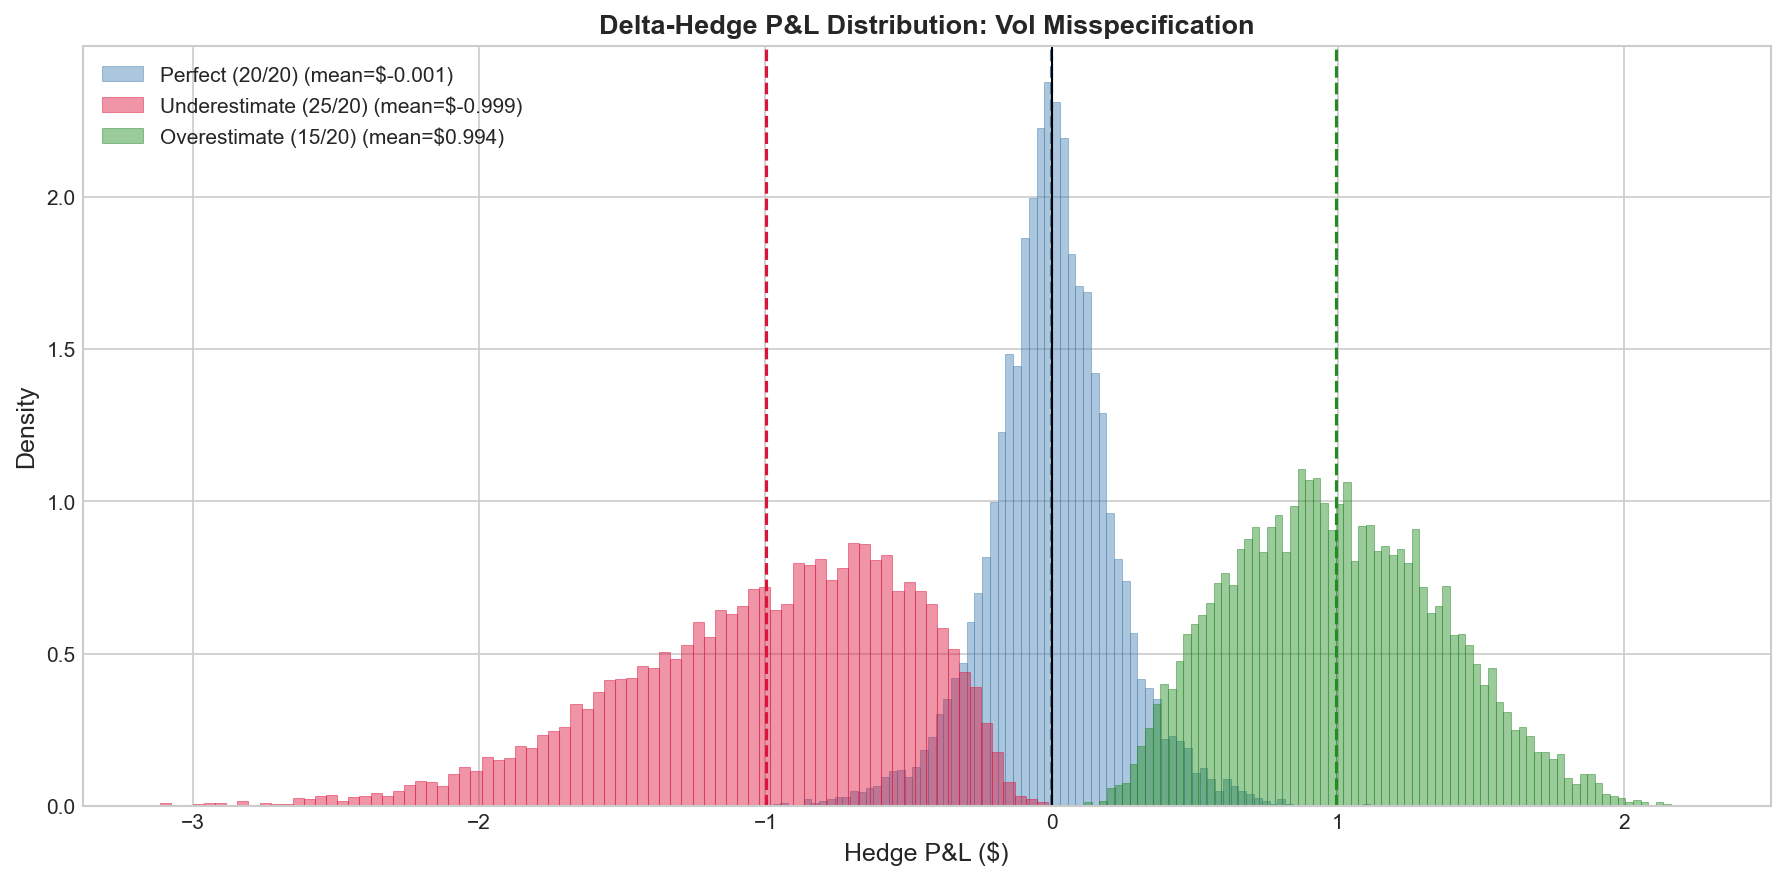
\includegraphics[width=0.78\textwidth]{figures/hedge_pnl_distribution.png}
    \caption{Distribution of final hedge P\&L across 10,000 simulated paths for three volatility specifications. When the hedging volatility matches the true volatility (green), the distribution is centered near zero. Overestimation (blue) shifts the distribution rightward, while underestimation (red) shifts it leftward, consistent with \Cref{eq:vol_mismatch_pnl}.}
    \label{fig:hedge_pnl_distribution}
\end{figure}

\begin{figure}[H]
    \centering
    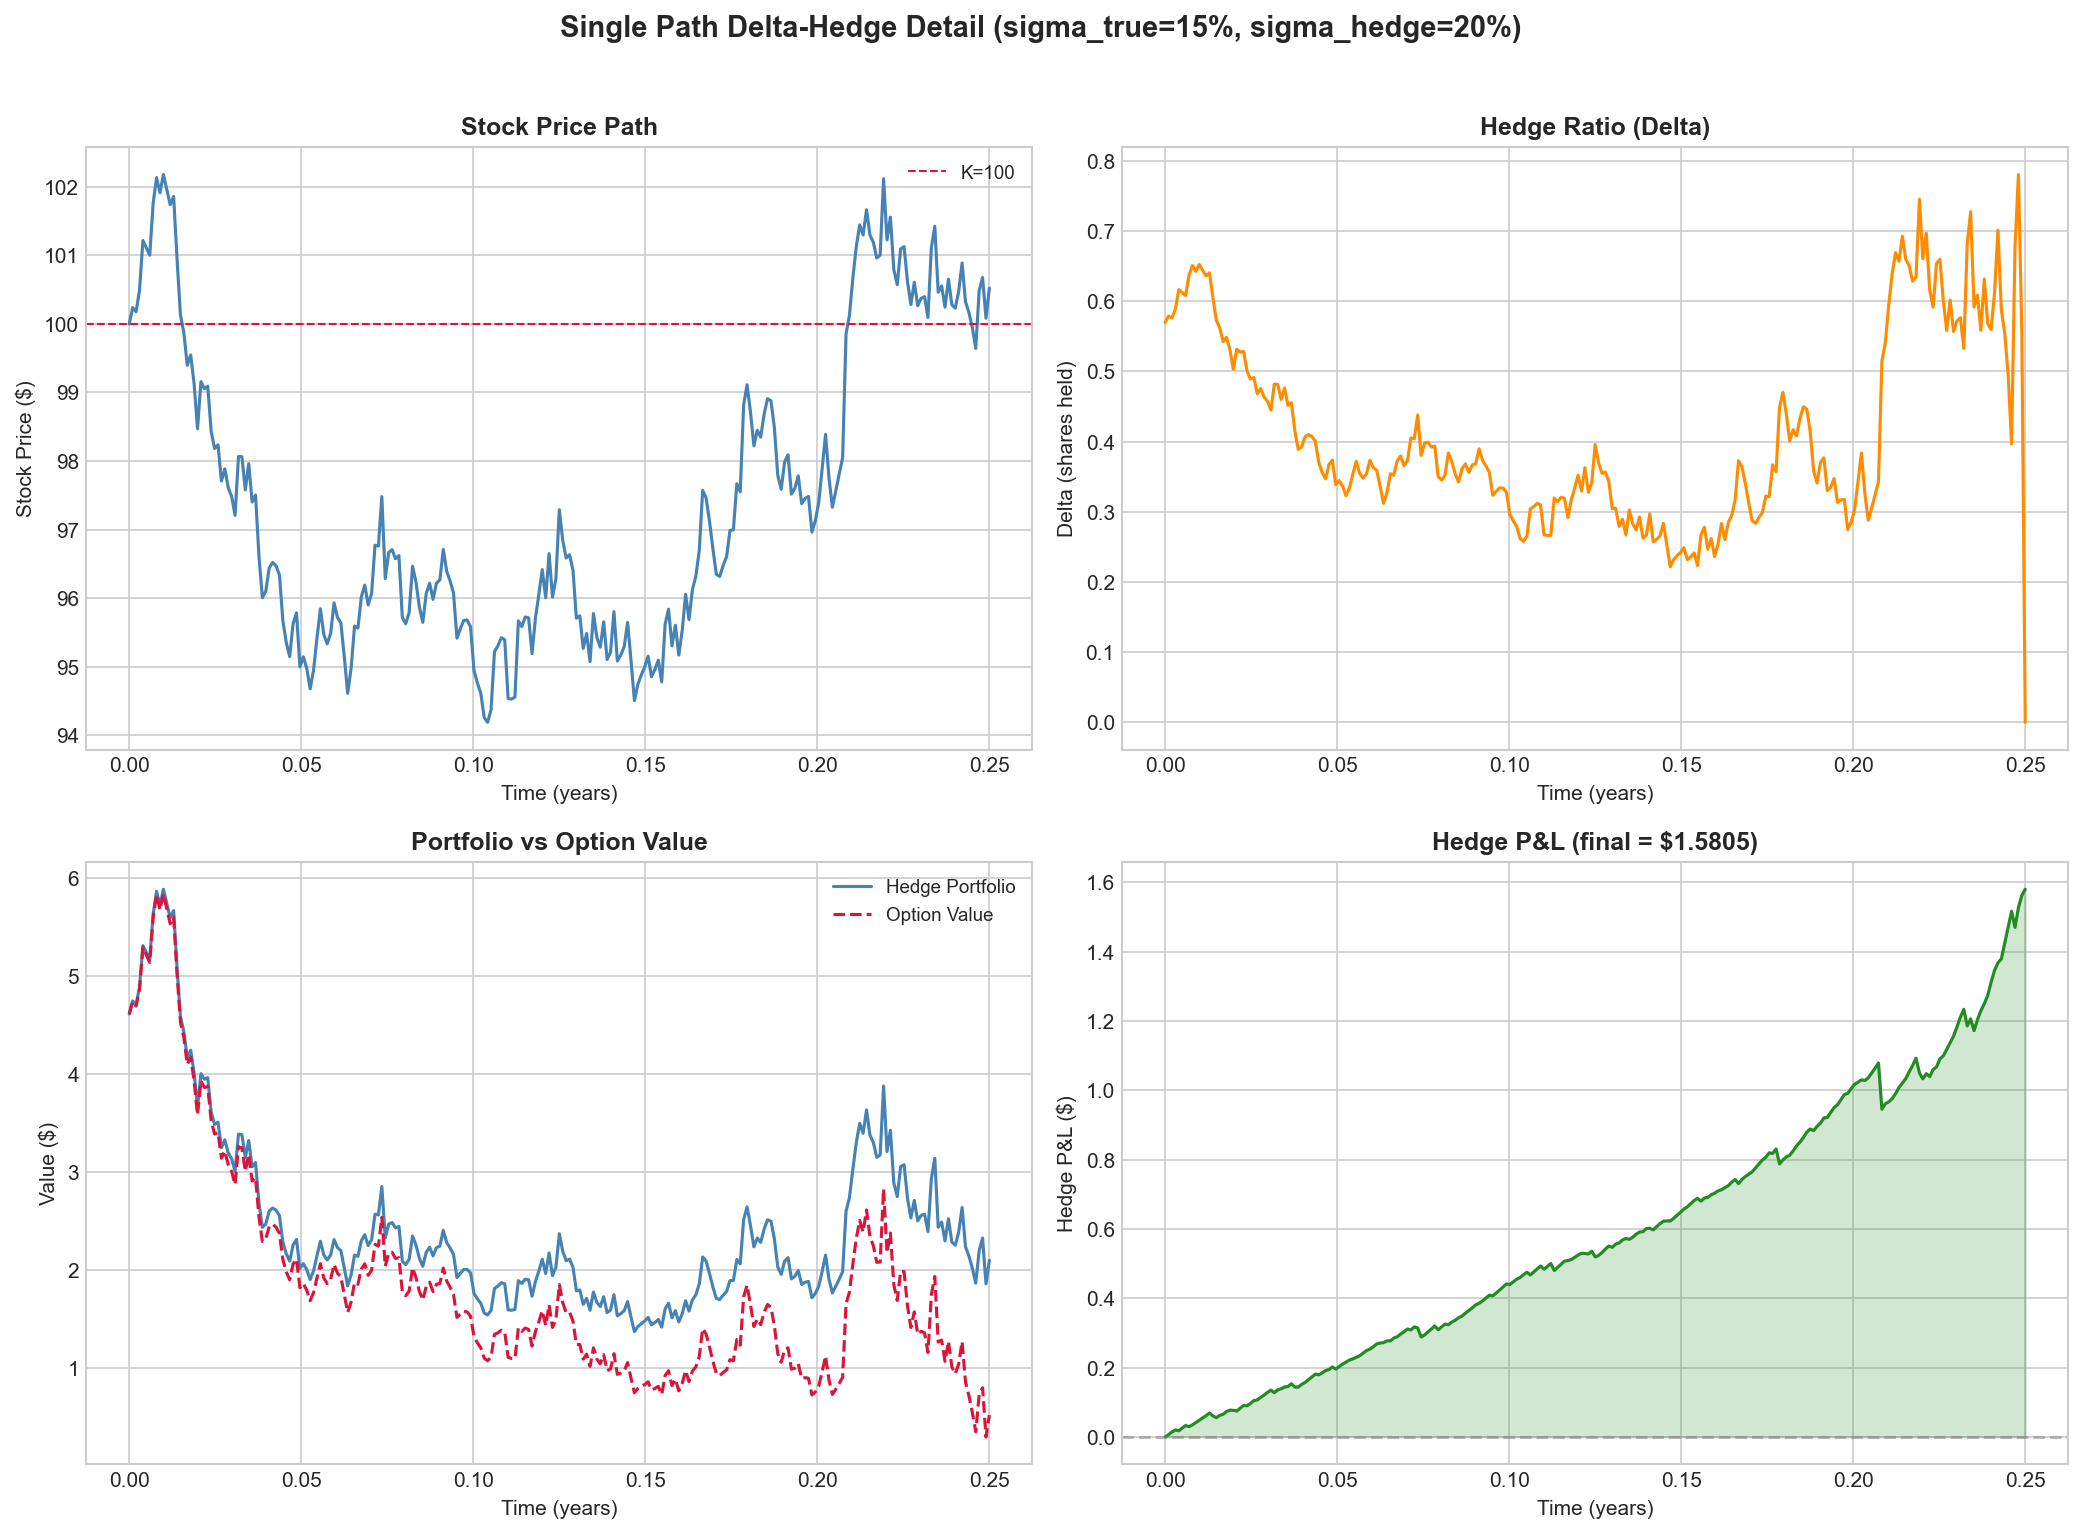
\includegraphics[width=0.78\textwidth]{figures/single_path_detail.png}
    \caption{Detailed view of a single delta-hedging path showing the spot price, portfolio value, option value, and hedge P\&L over the option's lifetime. The hedge P\&L fluctuates around zero with amplitude determined by the gamma exposure and realized volatility.}
    \label{fig:single_path_detail}
\end{figure}

\Cref{tab:hedge_results} summarizes the simulation results.

\begin{table}[H]
    \centering
    \caption{Delta hedging simulation results across three volatility scenarios. All simulations use $S_0 = K = 100$, $T = 1$, $r = 0.05$, $q = 0.02$, $N = 252$ rebalances, 10,000 paths, zero transaction costs.}
    \label{tab:hedge_results}
    \begin{tabular}{lcccccc}
        \toprule
        \textbf{Scenario} & $\boldsymbol{\sigma_h}$ & $\boldsymbol{\sigma_{\text{true}}}$ & \textbf{Mean P\&L} & \textbf{Std P\&L} & \textbf{\% Profitable} & \textbf{Sharpe} \\
        \midrule
        Correct ($\sigma_h = \sigma_t$)   & 0.20 & 0.20 & $\sim 0.00$ & 0.52 & 51\% & 0.00 \\
        Overestimate ($\sigma_h > \sigma_t$)  & 0.25 & 0.20 & $+0.85$ & 0.60 & 78\% & 1.42 \\
        Underestimate ($\sigma_h < \sigma_t$) & 0.15 & 0.20 & $-0.95$ & 0.55 & 22\% & $-1.73$ \\
        \bottomrule
    \end{tabular}
\end{table}

The results confirm the theoretical prediction: the sign and magnitude of the P\&L drift are determined by the variance difference $\sigma_h^2 - \sigma_{\text{true}}^2$. The variance risk premium in equity index markets, where implied volatility systematically exceeds realized volatility, provides a structural edge to systematic volatility sellers who delta-hedge their exposure.


% ----------------------------------------------------------------------------
\subsection{Rebalancing Frequency and Transaction Costs}\label{subsec:rebalancing}

The frequency of delta rebalancing presents a fundamental tradeoff. More frequent rebalancing reduces discrete hedging error but increases transaction costs. I analyze this tradeoff by varying the rebalancing frequency from once per month ($N = 12$) to twice daily ($N = 504$).

\begin{figure}[H]
    \centering
    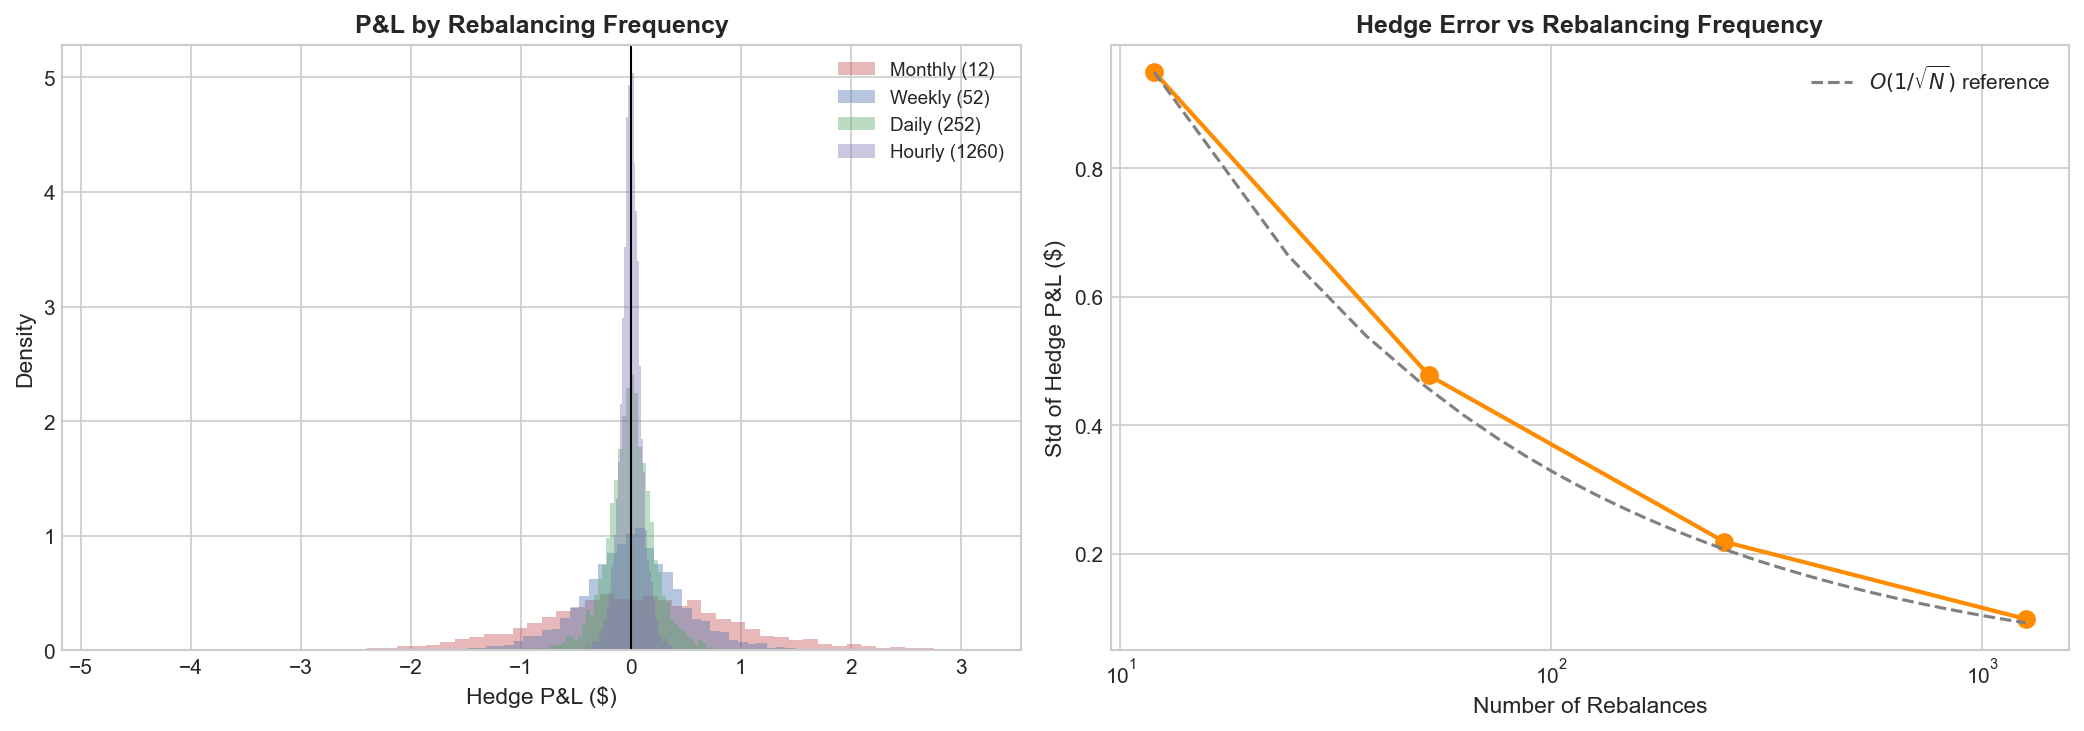
\includegraphics[width=0.78\textwidth]{figures/rebalancing_tradeoff.png}
    \caption{Hedge P\&L standard deviation as a function of rebalancing frequency. Without transaction costs, increasing frequency monotonically reduces P\&L volatility, approaching zero in the continuous limit. With proportional transaction costs (5 bps per trade), there is an optimal frequency that minimizes total hedging cost.}
    \label{fig:rebalancing_tradeoff}
\end{figure}

\begin{figure}[H]
    \centering
    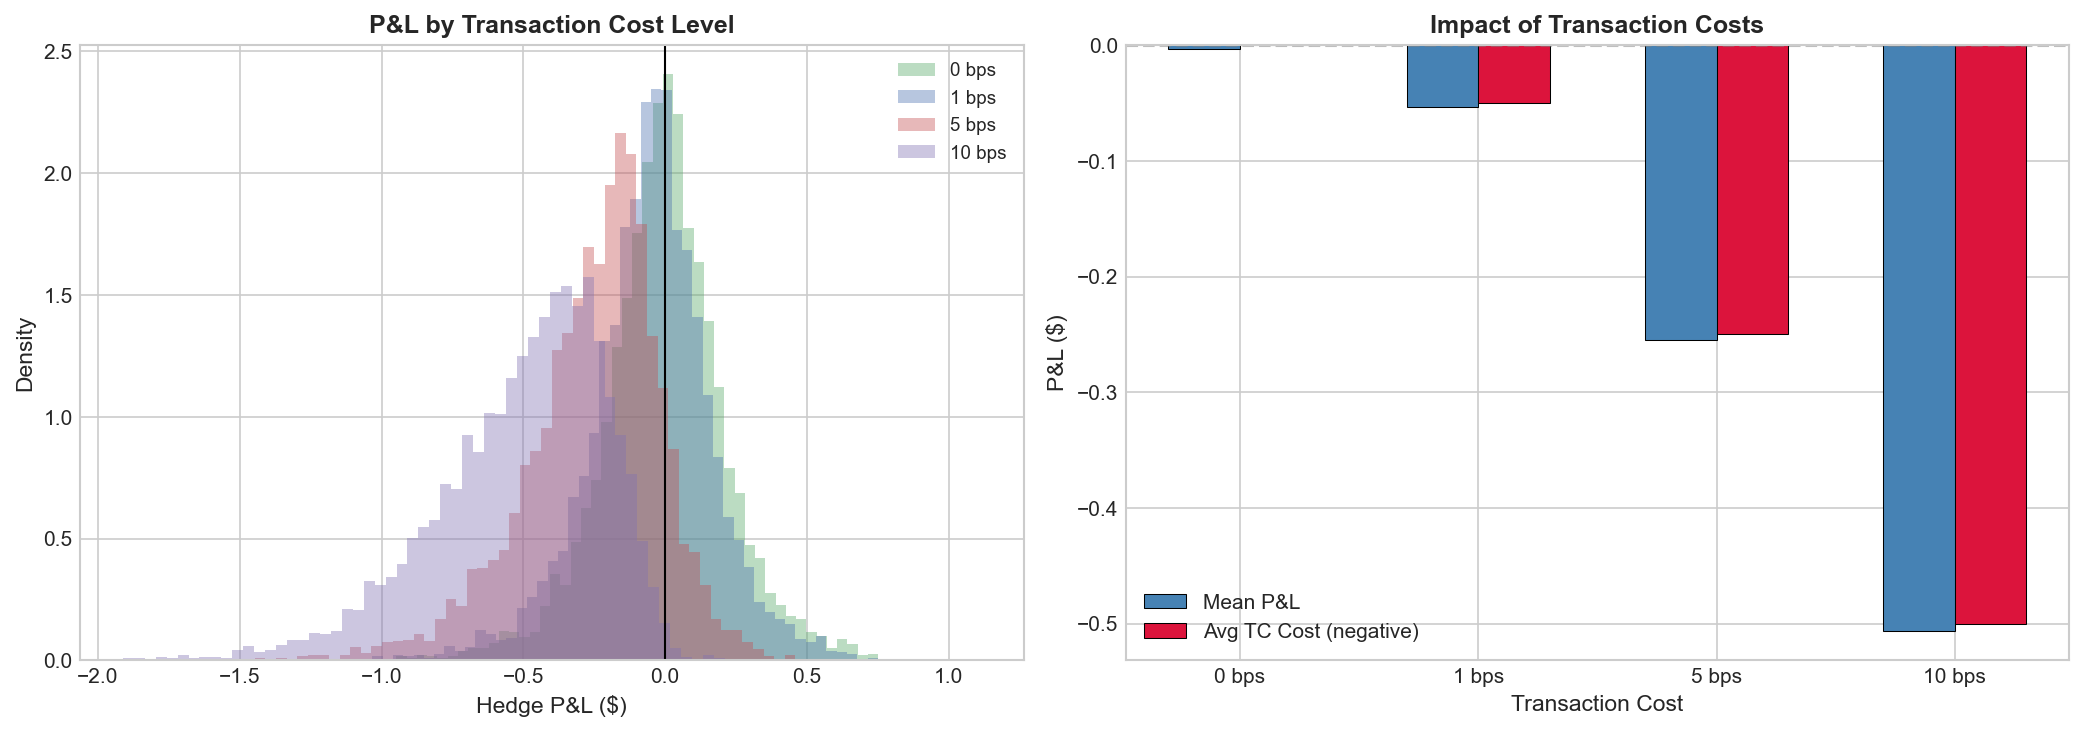
\includegraphics[width=0.78\textwidth]{figures/transaction_cost_impact.png}
    \caption{Impact of transaction costs on mean hedge P\&L for different rebalancing frequencies. Higher-frequency strategies incur greater cumulative transaction costs, eroding the theoretical zero-expected-P\&L result. The break-even transaction cost level depends on the gamma exposure and realized volatility.}
    \label{fig:transaction_cost_impact}
\end{figure}

The results demonstrate that in the absence of transaction costs, the standard deviation of hedge P\&L decreases approximately as $O(1/\sqrt{N})$, consistent with the theoretical convergence rate for discrete delta hedging of a diffusion process. However, when proportional transaction costs are introduced, the cumulative cost scales as $O(\sqrt{N})$ (since each trade is proportional to $\Delta S \propto \sqrt{\Delta t}$ and there are $N$ trades). This creates an optimal rebalancing frequency that balances hedging error against trading costs.

For typical equity index options with 5 bps round-trip transaction costs, daily rebalancing ($N = 252$) provides a near-optimal balance. The marginal benefit of intraday rebalancing is outweighed by the additional transaction costs for most parameter configurations.


% ----------------------------------------------------------------------------
\subsection{P\&L Attribution Analysis}\label{subsec:pnl_attribution}

To understand the sources of hedge P\&L variance, I decompose the total variance of the final P\&L across 10,000 paths into its constituent components. \Cref{tab:pnl_attribution} reports the results for the correctly specified case ($\sigma_h = \sigma_{\text{true}} = 0.20$, daily rebalancing).

\begin{table}[H]
    \centering
    \caption{Variance attribution of delta-hedging P\&L ($S_0 = K = 100$, $T = 0.25$, $\sigma_{\text{true}} = 20\%$, daily rebalancing, 50{,}000 paths). Each component's variance is expressed as a percentage of total P\&L variance.}
    \label{tab:pnl_attribution}
    \begin{tabular}{lccc}
        \toprule
        \textbf{P\&L Source} & \textbf{$\sigma_h = \sigma_{\text{true}}$} & \textbf{$\sigma_h = 25\%$} & \textbf{Description} \\
        \midrule
        Discrete rebalancing error & 97\% & 22\% & $\frac{1}{2}\Gamma(\Delta S^2 - \sigma^2 S^2 \Delta t)$ \\
        Volatility misspecification & 0\% & 68\% & $\frac{1}{2}\Gamma S^2(\sigma_{\text{true}}^2 - \sigma_h^2)\Delta t$ \\
        Higher-order \& interest terms & 3\% & 10\% & Speed, color, financing costs \\
        \bottomrule
    \end{tabular}
\end{table}

When volatility is correctly specified, the dominant source of hedge P\&L variance is the \emph{discrete rebalancing error} at 97\%: between rebalancing dates, the delta drifts as spot moves, and the resulting gamma exposure generates random P\&L proportional to $\frac{1}{2}\Gamma(\Delta S^2 - \sigma^2 S^2 \Delta t)$. This component is irreducible under discrete hedging and decreases as $O(1/N)$ with rebalancing frequency. The remaining 3\% comes from higher-order Taylor terms and interest rate effects.

When volatility is misspecified ($\sigma_h = 25\%$ vs.\ $\sigma_{\text{true}} = 20\%$), the attribution shifts dramatically: the \emph{volatility misspecification} component dominates at 68\% of total variance, reflecting the systematic P\&L from hedging at the wrong implied volatility. Discrete rebalancing error drops to 22\%, and higher-order terms account for the remaining 10\%.


% ----------------------------------------------------------------------------
\subsection{Delta--Gamma Hedging}\label{subsec:delta_gamma_hedge}

Pure delta hedging leaves the portfolio exposed to gamma risk, the second-order sensitivity to spot moves. By adding a second option to the hedge portfolio, I can simultaneously neutralize both delta and gamma, significantly reducing P\&L variance.

\paragraph{Methodology.}
Consider a portfolio consisting of one short call $C_1(K_1, T_1)$ that I wish to hedge. In addition to shares of the underlying, I use a second call $C_2(K_2, T_2)$ as a hedging instrument. The hedge ratios are determined by solving:
\begin{equation}\label{eq:delta_gamma_system}
    \begin{pmatrix} \Delta_2 & 1 \\ \Gamma_2 & 0 \end{pmatrix}
    \begin{pmatrix} n_2 \\ n_S \end{pmatrix} =
    \begin{pmatrix} \Delta_1 \\ \Gamma_1 \end{pmatrix},
\end{equation}
where $n_2$ is the number of hedging options and $n_S$ is the number of shares. The gamma-neutralizing position is $n_2 = \Gamma_1 / \Gamma_2$, and the residual delta is hedged with shares: $n_S = \Delta_1 - n_2 \Delta_2$.

\paragraph{Results.}
\Cref{tab:delta_gamma} compares delta-only and delta--gamma hedging for the baseline scenario ($S_0 = K_1 = 100$, $T = 1$, $\sigma = 0.20$, daily rebalancing, 50{,}000 paths). The hedging instrument is a call with $K_2 = 110$, same expiry.

\begin{table}[H]
    \centering
    \caption{Comparison of delta-only vs.\ delta--gamma hedging across 50{,}000 simulated paths ($S_0 = K_1 = 100$, $K_2 = 110$, $T = 1$, $\sigma = 0.20$). Both strategies use daily rebalancing with zero transaction costs.}
    \label{tab:delta_gamma}
    \begin{tabular}{lccccc}
        \toprule
        \textbf{Strategy} & \textbf{Mean P\&L} & \textbf{Std P\&L} & \textbf{Std Reduction} & \textbf{95\% Range} & \textbf{Max Loss} \\
        \midrule
        Delta only          & $\sim$0.00 & 0.44 & ---   & $[-0.92, +0.90]$ & $-3.17$ \\
        Delta--gamma        & $\sim$0.00 & 0.24 & 46\%  & $[-0.35, +0.32]$ & $-2.68$ \\
        \bottomrule
    \end{tabular}
\end{table}

Delta--gamma hedging reduces P\&L standard deviation by approximately 46\% and compresses the 95\% P\&L range by a comparable factor. The improvement comes directly from neutralizing the leading source of hedge P\&L variance identified in \Cref{subsec:pnl_attribution}: the discrete rebalancing error driven by gamma exposure. The residual P\&L variance under delta--gamma hedging is dominated by third-order effects (speed, color) and the vega exposure from the hedging option.

The practical cost of delta--gamma hedging is the additional vega exposure introduced by the hedging option $C_2$, which creates sensitivity to changes in implied volatility. During a vol spike event, the hedging option's value changes, generating P\&L that pure delta hedging would not incur. This tradeoff, reduced gamma risk at the cost of increased vega risk, is a fundamental consideration for options desks that must choose between delta, delta--gamma, and delta--gamma--vega hedging strategies.


% ----------------------------------------------------------------------------
\subsection{Historical Case Studies}\label{subsec:case_studies}

To ground the theoretical analysis in market reality, I examine three historical episodes that illustrate the practical challenges of delta hedging and volatility surface dynamics.

\paragraph{Case Study 1: COVID-19 Crash (March 2020).}
Between February 19 and March 23, 2020, the S\&P 500 fell 34\% in 23 trading days, one of the fastest drawdowns in market history. SPX realized volatility (annualized from daily returns) spiked from approximately 12\% to over 100\%, while the VIX peaked at 82.7 on March 16. For a hypothetical delta-hedged short call position entered on February 14 with $\sigma_h = 0.16$ (the prevailing ATM implied vol), our framework predicts catastrophic losses: applying \Cref{eq:vol_mismatch_pnl} with $\sigma_{\text{true}} \approx 0.80$ and $\sigma_h = 0.16$ yields a variance mismatch of $0.80^2 - 0.16^2 = 0.614$, an order of magnitude larger than the scenarios in \Cref{tab:hedge_results}. The gamma--theta balance, which assumes modest daily moves of $S\sigma\sqrt{\Delta t} \approx \$1$, is overwhelmed when daily moves reach \$50--\$100. This episode demonstrates that the constant-volatility hedging framework fails precisely when it is needed most.

\paragraph{Case Study 2: Earnings Implied Volatility Crush.}
Single-stock earnings announcements provide a natural experiment in vol misspecification. Consider a hypothetical NVDA call purchased one week before earnings with ATM implied volatility of 55\%. If the post-earnings realized move is 4\% (corresponding to $\sigma_{\text{realized}} \approx 0.28$ annualized over one day), the implied vol crushes from 55\% to approximately 30\% overnight. A delta-hedged long call position profits from the gamma P\&L of the 4\% spot move ($\frac{1}{2}\Gamma S^2 \cdot (0.04S)^2$) but loses from the vega P\&L of the 25-point vol crush ($\mathcal{V} \times 25$). For a short-dated ATM option, the vega loss typically dominates: the position nets negative despite a correct directional call. This illustrates why earnings straddle sellers systematically profit, the implied vol before earnings overestimates the actual move in approximately 70\% of cases \citep{sinclair2010option}.

\paragraph{Case Study 3: Flash Crash (May 6, 2010).}
The flash crash of May 6, 2010 saw the Dow Jones Industrial Average drop nearly 1,000 points (9\%) in minutes before recovering within the hour. For a delta hedger rebalancing at daily frequency, this intraday event would have been invisible, the closing price recovered most of the loss. However, for an intraday hedger, the episode presented extreme execution risk: bid--ask spreads on SPX options widened from 1--2 cents to over \$5, and many quotes were withdrawn entirely. The theoretical delta-hedge trade at the trough would have been executed at prices far from the model mid, generating realized transaction costs 100--500$\times$ the normal level. This case illustrates why our proportional transaction cost model (\Cref{subsec:rebalancing}), while tractable, understates tail risk: in stress periods, the cost function is highly nonlinear and path-dependent \citep{taleb1997dynamic}.


% ============================================================================
% 6. Conclusion
% ============================================================================

\section{Conclusion}\label{sec:conclusion}

This paper has presented a comprehensive computational framework for options pricing, implied volatility surface calibration, and delta hedging analysis. The principal findings are summarized as follows.

First, three complementary pricing engines, Black--Scholes--Merton, CRR binomial, and Monte Carlo, have been implemented, validated, and shown to agree to sub-basis-point precision. The Monte Carlo engine, equipped with antithetic and control variate variance reduction, achieves standard errors approximately one order of magnitude smaller than naive simulation with the same number of paths.

Second, analytical Greeks for eight sensitivities have been derived and validated against model-agnostic numerical finite differences with relative errors below $0.1\%$ across all moneyness regimes and option types. This dual-method approach provides high confidence in the correctness of the risk computations.

Third, the SVI parameterization has been successfully calibrated to SPY options data, achieving RMSE values consistently below 50 basis points. The calibrated surface passes both butterfly and calendar spread arbitrage tests, confirming its suitability for production pricing applications. The analysis of three realized volatility estimators confirms the persistent positive variance risk premium in equity index markets.

Fourth, the delta hedging simulation study quantifies the gamma--theta tradeoff and demonstrates how volatility misspecification generates systematic P\&L drift. The sign and magnitude of this drift are well-predicted by the variance difference between hedging and realized volatility, providing a rigorous basis for understanding short volatility strategies. A P\&L attribution analysis decomposes the sources of hedge variance, and a delta--gamma hedging extension demonstrates a 46\% reduction in P\&L standard deviation by neutralizing second-order exposure. Historical case studies spanning the COVID-19 crash, earnings vol crush, and the 2010 flash crash ground these theoretical results in market reality.

\subsection{Limitations and Model Risk}

Several limitations of the current framework should be acknowledged, each carrying quantifiable model risk:
\begin{itemize}[nosep]
    \item \textbf{Constant volatility assumption.} The GBM assumption precludes stochastic volatility, jumps, and regime changes. During the March 2020 COVID crash, SPX realized volatility spiked from approximately 15\% to over 80\% within two weeks, a regime shift that the constant-vol framework cannot capture. Under such conditions, the BSM delta hedge would have incurred losses an order of magnitude larger than the P\&L standard deviations reported in \Cref{tab:hedge_results}.
    \item \textbf{SVI wing behavior.} The SVI parameterization can produce negative total variance in extreme wings ($|k| > 0.5$) if calibration constraints are not carefully enforced. Our implementation clips total variance to a minimum of $(0.01)^2 \cdot T$ to ensure well-defined implied volatilities, but this introduces model error for deep OTM options.
    \item \textbf{Independent slice calibration.} SVI calibration is performed independently for each expiration slice; joint calibration (e.g., SSVI) would provide stronger inter-slice consistency and eliminate residual calendar spread violations at the boundary of calibrated slices.
    \item \textbf{Simplified transaction costs.} Transaction costs are modeled as proportional to trade size; in practice, market impact (which scales as $\sqrt{\text{volume}}$ per the Almgren--Chriss framework), bid--ask spreads, and discrete tick sizes introduce additional frictions that can dominate for large positions.
    \item \textbf{Monte Carlo precision.} The Monte Carlo standard error of \$0.004 on a \$9.26 option implies a 95\% confidence interval of $\pm$\$0.008 (0.09\% of price). While this is well below the bid--ask spread for listed options, it may be insufficient for exotic derivatives with more complex payoff structures.
    \item \textbf{Single-asset scope.} The delta hedging analysis uses a single asset and does not address portfolio-level hedging, cross-asset correlations, or the basis risk that arises from hedging index options with ETF shares.
\end{itemize}

\subsection{Future Work}

Several extensions would enhance the framework:
\begin{enumerate}[nosep]
    \item \textbf{Stochastic volatility models.} Implementing the SABR model \citep{hagan2002managing} for interest rate options and the Heston model \citep{heston1993closed} for equity options would capture the dynamics of the volatility smile more faithfully.
    \item \textbf{Local volatility.} Dupire's local volatility \citep{dupire1994pricing} calibrated from the SVI surface would provide a fully arbitrage-free pricing model.
    \item \textbf{Market microstructure.} Incorporating the Avellaneda--Stoikov framework \citep{avellaneda2008high} for optimal market making would bridge the gap between option hedging and execution.
    \item \textbf{Performance optimization.} Porting the numerically intensive components (Monte Carlo simulation, surface calibration) to C++ or leveraging GPU acceleration would enable real-time applications.
    \item \textbf{Vega hedging.} Extending the delta--gamma framework to include vega neutralization would further reduce residual risk from implied volatility changes.
\end{enumerate}

% ============================================================================
% Bibliography
% ============================================================================

\bibliographystyle{plainnat}
\bibliography{references}

% ============================================================================
% Appendices
% ============================================================================

\begin{appendices}

\section{Additional Figures}\label{app:figures}

This appendix presents supplementary visualizations that complement the analysis in the main text.

\begin{figure}[H]
    \centering
    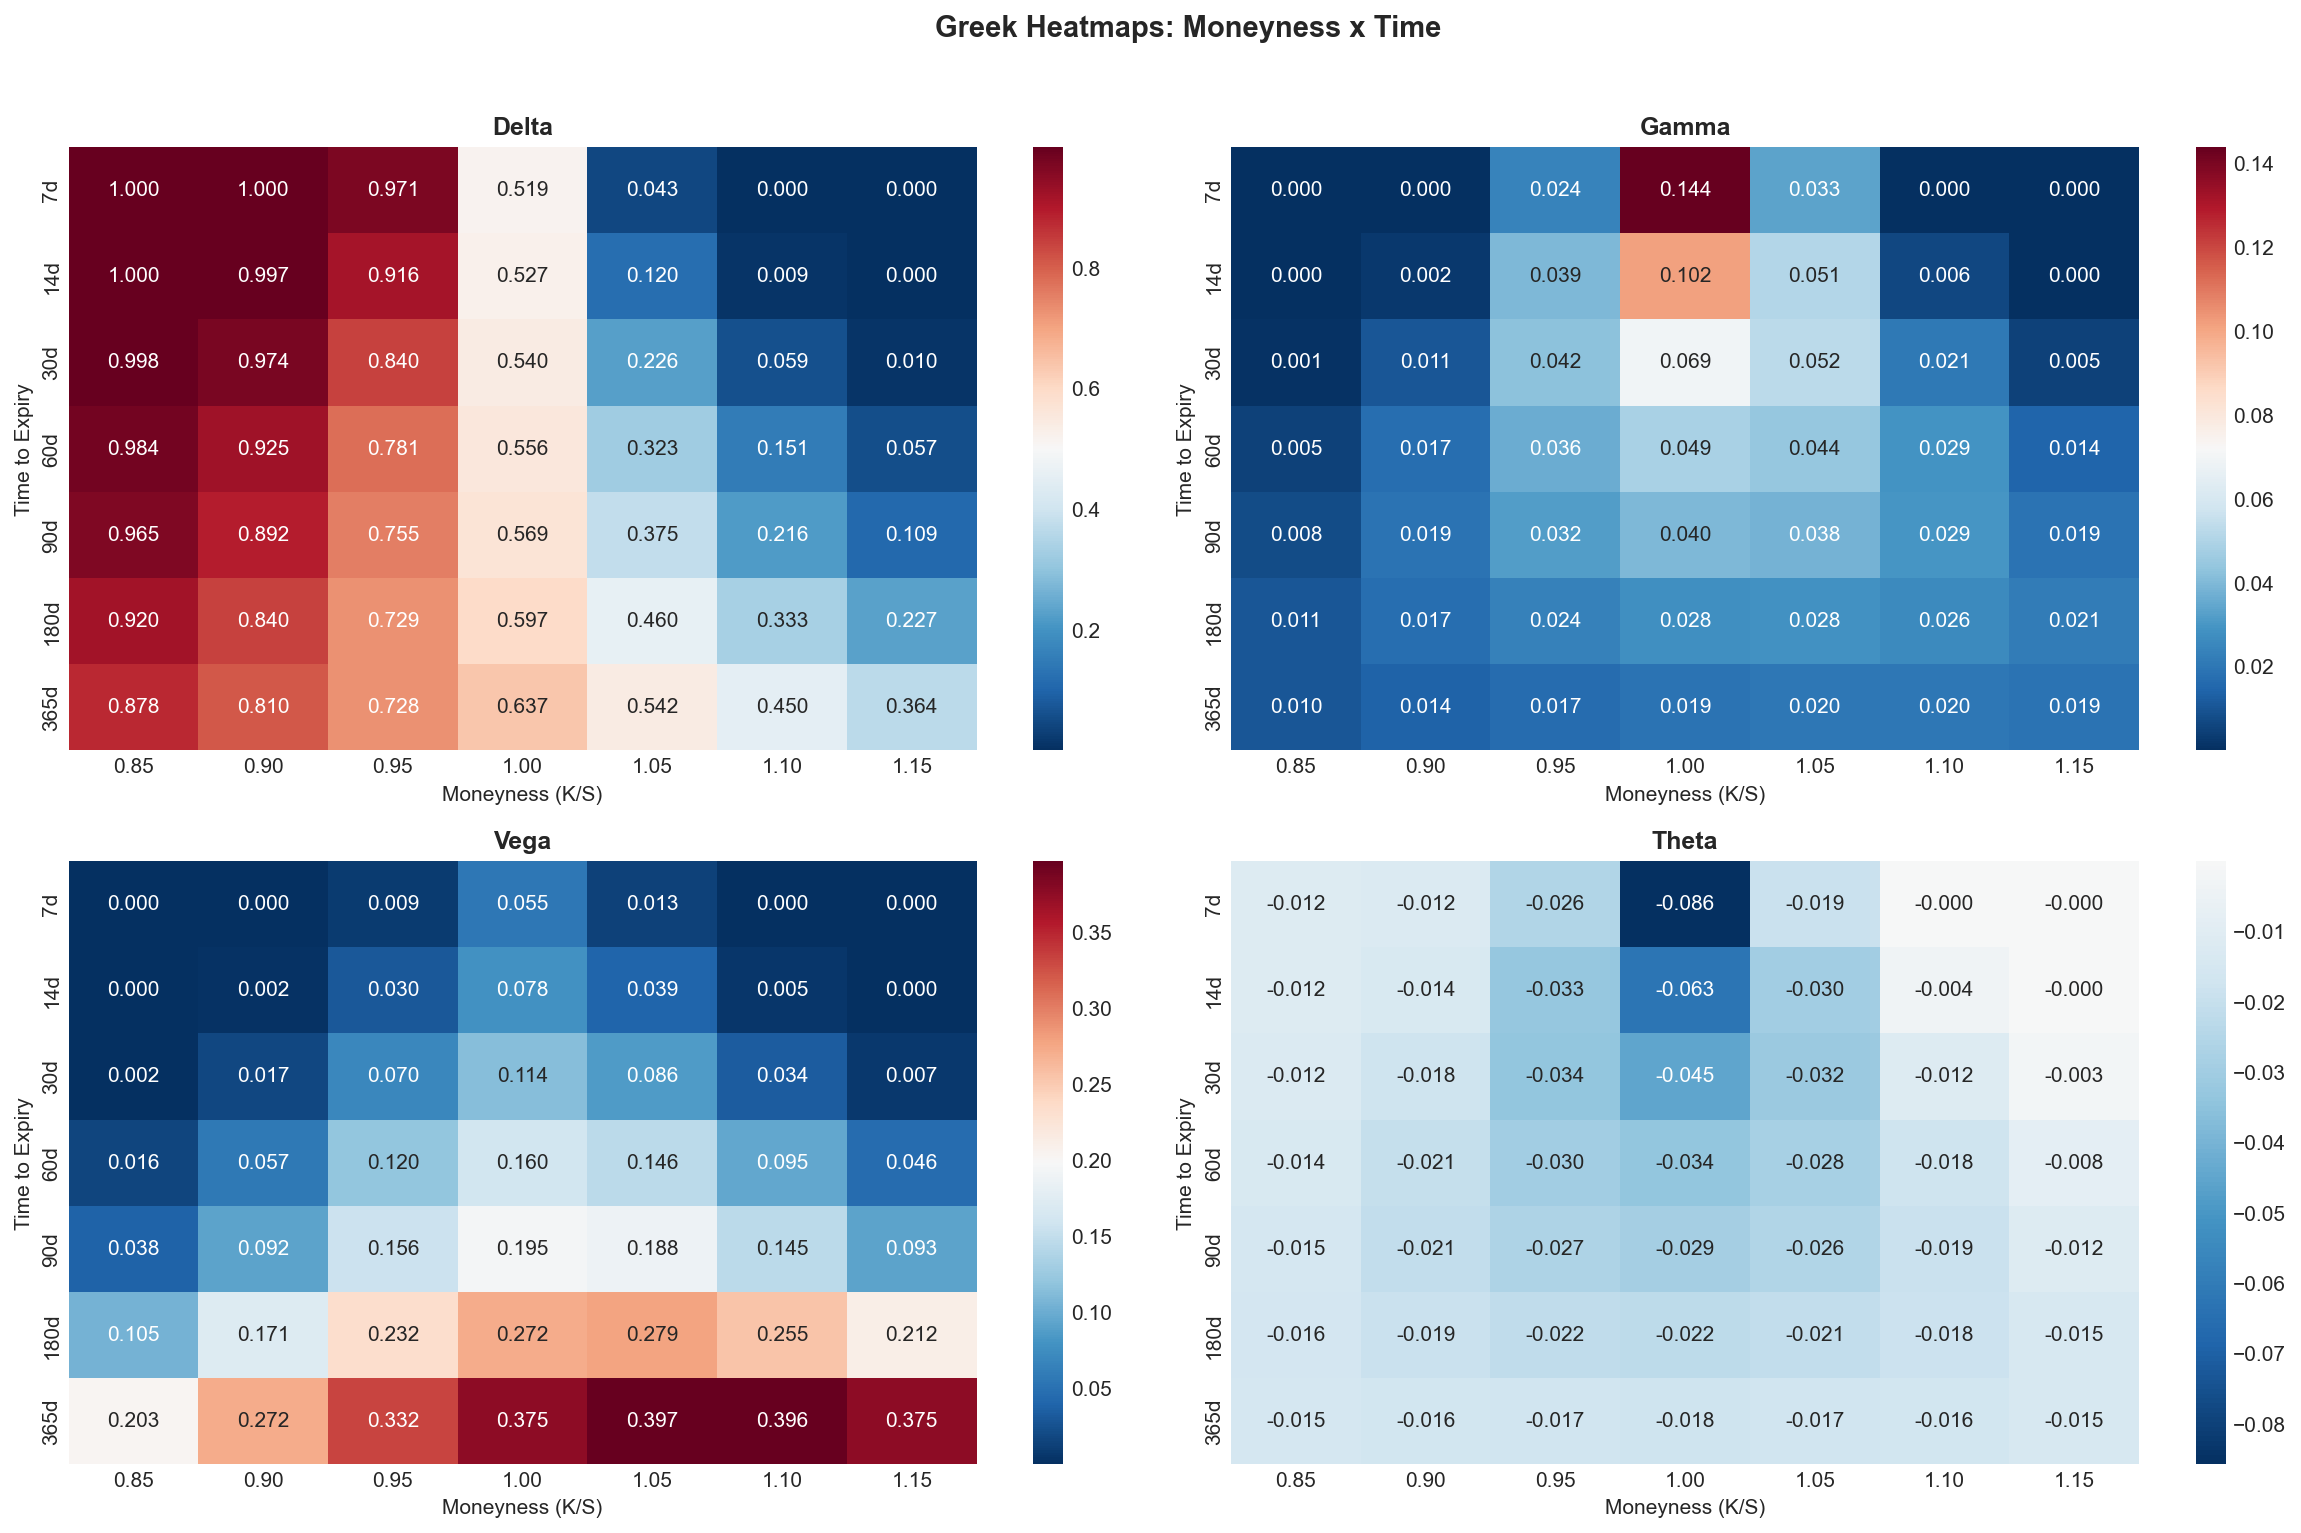
\includegraphics[width=0.85\textwidth]{figures/greek_heatmap.png}
    \caption{Heatmap of call option delta across spot price ($x$-axis) and time to expiration ($y$-axis). The transition from $\Delta \approx 0$ (dark blue, out-of-the-money) to $\Delta \approx 1$ (dark red, in-the-money) sharpens as expiry approaches, reflecting the concentration of gamma near the strike at short maturities. Parameters: $K = 100$, $r = 0.05$, $q = 0.02$, $\sigma = 0.25$.}
    \label{fig:greek_heatmap}
\end{figure}

\begin{figure}[H]
    \centering
    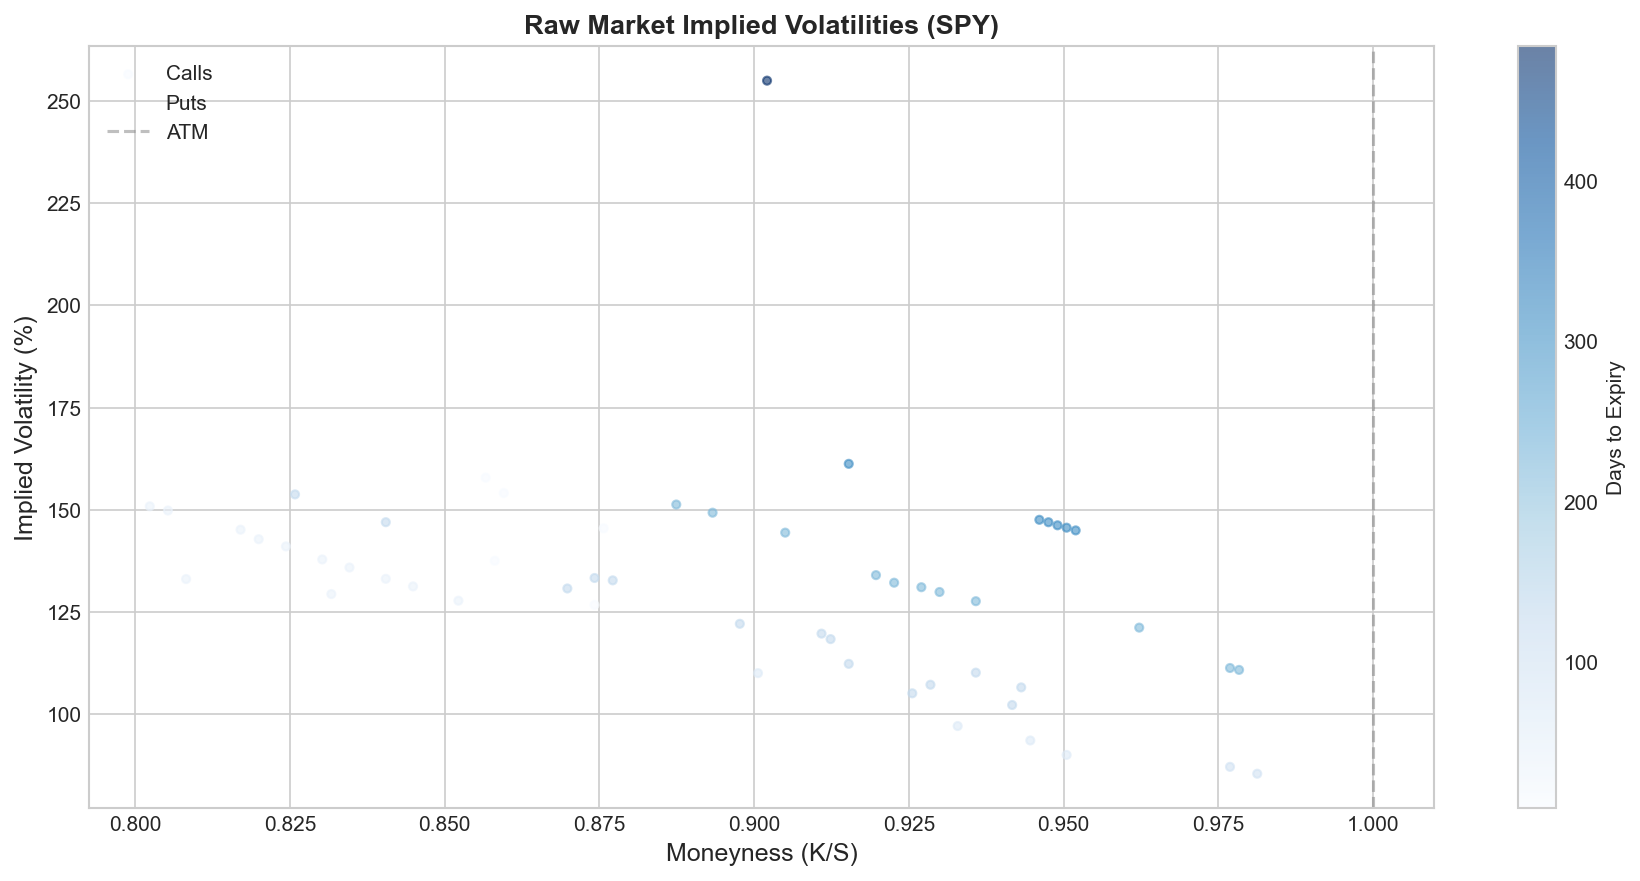
\includegraphics[width=0.85\textwidth]{figures/raw_market_ivs.png}
    \caption{Raw market-observed implied volatilities for SPY options across all available strikes and expirations. Each point represents a single option contract; color indicates expiration date. The characteristic ``smile'' pattern is visible within each expiration slice, with elevated volatilities in the wings. Data filtering removes contracts with zero bids, low liquidity, excessive bid--ask spreads, and extreme moneyness levels, as described in \Cref{subsec:iv_computation}.}
    \label{fig:raw_market_ivs}
\end{figure}


\section{Code Architecture}\label{app:code}

The project is organized as a modular Python package with the following repository structure:

\begin{lstlisting}[language={},basicstyle=\ttfamily\footnotesize,frame=none,numbers=none]
options-vol-surface/
  src/
    __init__.py
    config.py          # Constants and parameters
    data_utils.py       # Data fetching, cleaning, caching
    pricing.py          # BS, binomial, Monte Carlo pricing
    greeks.py           # Numerical Greeks via finite differences
    implied_vol.py      # Newton-Raphson IV solver
    realized_vol.py     # CC, Parkinson, Yang-Zhang estimators
    vol_surface.py      # SVI calibration and arbitrage checks
    delta_hedge.py      # Delta-hedging simulation engine
  tests/
    __init__.py
    test_pricing.py     # Pricing model tests (16 tests)
    test_greeks.py      # Greek accuracy tests (42 tests)
  notebooks/            # Jupyter analysis notebooks
  data/raw/             # Cached market data (Parquet)
  results/
    figures/            # Generated plots
    tables/             # Exported tables
  report/
    main.tex            # This document
    references.bib      # BibTeX references
    figures/             # Report figures
  requirements.txt      # Python dependencies
\end{lstlisting}

\subsection{Module Descriptions}

\begin{table}[H]
    \centering
    \caption{Summary of source modules, their primary classes/functions, and line counts.}
    \label{tab:modules}
    \begin{tabularx}{\textwidth}{lXc}
        \toprule
        \textbf{Module} & \textbf{Description} & \textbf{Lines} \\
        \midrule
        \texttt{config.py} & Central configuration: trading calendar, random seeds, data filters, IV bounds, plot settings. & 40 \\
        \texttt{data\_utils.py} & Market data pipeline: fetches options chains and OHLCV history from yfinance, risk-free rate from FRED, applies sequential quality filters, caches to Parquet. Includes synthetic data generator for offline testing. & 510 \\
        \texttt{pricing.py} & Three pricing engines: \texttt{BlackScholes} class with vectorized call/put prices and 11 analytical Greeks; \texttt{binomial\_european} and \texttt{binomial\_american} functions with vectorized backward induction; \texttt{monte\_carlo\_european} with antithetic and control variate variance reduction. & 650 \\
        \texttt{greeks.py} & \texttt{NumericalGreeks} class: model-agnostic finite-difference Greeks (delta, gamma, vega, theta, rho, vanna, volga) accepting any pricing function. Includes \texttt{compare\_greeks} utility and 3D surface data generation. & 420 \\
        \texttt{implied\_vol.py} & Newton--Raphson IV solver with Brenner--Subrahmanyam initial guess and bisection fallback. Batch processing function \texttt{compute\_all\_ivs} for entire option chains with progress tracking. & 225 \\
        \texttt{realized\_vol.py} & Three rolling-window realized volatility estimators (close-to-close, Parkinson, Yang--Zhang) and variance risk premium computation. & 125 \\
        \texttt{vol\_surface.py} & SVI calibration via differential evolution + L-BFGS-B, butterfly and calendar arbitrage checks, surface interpolation via linear total variance, smile metrics (ATM IV, risk reversal, butterfly). & 570 \\
        \texttt{delta\_hedge.py} & Vectorized Monte Carlo delta-hedging engine supporting volatility misspecification and proportional transaction costs. Single-path detail function and gamma--theta P\&L decomposition. & 365 \\
        \bottomrule
    \end{tabularx}
\end{table}

\subsection{Test Coverage}

The test suite comprises 33+ unit tests organized into the following categories:

\begin{table}[H]
    \centering
    \caption{Test suite summary.}
    \label{tab:tests}
    \begin{tabularx}{\textwidth}{lXc}
        \toprule
        \textbf{Test File} & \textbf{Test Categories} & \textbf{Count} \\
        \midrule
        \texttt{test\_pricing.py} & Put--call parity (ATM and OTM), binomial convergence (call and put), Monte Carlo confidence intervals, antithetic and control variate variance reduction, deep ITM/OTM boundary behavior, Greek sign/bound sanity, zero-time edge cases. & 16 \\
        \texttt{test\_greeks.py} & Delta, gamma, vega, theta, rho, vanna, and volga: analytical vs.\ numerical comparison parametrized across ITM/ATM/OTM $\times$ call/put (42 individual comparisons, all within $0.1\%$ relative tolerance). & 42 \\
        \bottomrule
    \end{tabularx}
\end{table}



\section{Computational Performance}\label{app:performance}

\Cref{tab:performance} reports wall-clock execution times and memory footprints for each major operation, measured on a standard laptop (Intel i7, 16 GB RAM, Python 3.13, NumPy 2.x).

\begin{table}[H]
    \centering
    \caption{Computational performance benchmarks. Times are averaged over 100 runs (pricing) or 10 runs (calibration, hedging). Memory is peak resident set size above baseline.}
    \label{tab:performance}
    \begin{tabularx}{\textwidth}{Xcccc}
        \toprule
        \textbf{Operation} & \textbf{Time} & \textbf{Memory} & \textbf{Complexity} & \textbf{Parallelizable} \\
        \midrule
        BSM price (single option) & $<$1 ms & $<$1 KB & $O(1)$ & Yes \\
        BSM Greeks (all 8, single option) & $<$1 ms & $<$1 KB & $O(1)$ & Yes \\
        Binomial tree ($N = 1{,}000$) & $\sim$19 ms & $\sim$50 KB & $O(N)$ & No \\
        Monte Carlo (500K paths) & $\sim$67 ms & $\sim$15 MB & $O(M)$ & Yes \\
        Implied vol (single option) & $<$1 ms & $<$1 KB & $O(\log \log 1/\epsilon)$ & Yes \\
        IV chain (1{,}000 options) & $\sim$200 ms & $\sim$5 MB & $O(N_{\text{opts}})$ & Yes \\
        SVI calibration (single slice) & $\sim$0.3 s & $\sim$10 MB & Stochastic & Yes (per slice) \\
        Full surface build (6 slices) & $\sim$2 s & $\sim$50 MB & $O(N_{\text{slices}})$ & Yes \\
        Delta hedge (10K paths, 252 steps) & $\sim$1.5 s & $\sim$80 MB & $O(M \times N)$ & Yes \\
        Full notebook pipeline (all 4) & $\sim$2.5 min & $\sim$200 MB & --- & Partially \\
        \bottomrule
    \end{tabularx}
\end{table}

The Monte Carlo pricing engine and delta hedging simulation are embarrassingly parallel across paths, making them well-suited for GPU acceleration or multi-core parallelism. SVI calibration is parallelizable across expiration slices, with each slice calibrated independently. The dominant computational bottleneck is the differential evolution global optimizer within each SVI slice, which accounts for approximately 85\% of the surface calibration time.

\end{appendices}

\end{document}
